\chapter{การวิเคราะห์และออกแบบระบบ}

การวิเคราะห์และออกแบบระบบก่อนดำเนินการจริงเป็นอีกหนึ่งขั้นตอนที่มีความสำคัญมาก เพราะการวิเคราะห์และออกแบบระบบนั้นเป็นการกระทำที่ทำให้ผู้พัฒนาเห็นรายละเอียดส่วนย่อยของงานทั้งหมด เพิ่มประสิทธิภาพในการวางแผน การทำงาน และยังช่วยลดปัญหาที่อาจจะเกิดขึ้นในระหว่างพัฒนา เพื่อให้ระบบมีความสมบูรณ์มากยิ่งขึ้น เนื่องจากการวิเคราะห์และออกแบบระบบนั้นจะช่วยให้ให้บริการ จัดการทรัพยากรได้อย่างคุ้มค่าและตรงตามความต้องการของระบบ

การวิเคราะห์และออกแบบแอปพลิเคชันสูงวัยมายเฟรนด์ ในบทนี้จะแบ่งออกเป็น 6 ขั้นตอนเพื่อให้เห็นการดำเนินงานอย่างมีระบบ ในหัวข้อแรกจะนำเสนอภาพรวมของระบบ ก่อนจะนำเสนอเอกสารแสดงความต้องการของระบบซึ่งจะทำให้เห็นที่มาของเพจต่าง ๆ ในขั้นตอนของการออกแบบในหัวข้อที่สาม ส่วนหัวข้อที่เหลือจะแสดงแผนภาพการการทำงานของระบบโดยใช้ UML diagram ซึ่งประกอบไปด้วย Use Case, Class และ Sequence Diagram เพื่อแสดงรายละเอียดของระบบก่อนนำไปเขียนคำสั่งด้วยภาษาโปรแกรมในบทต่อไป

\begin{enumerate}[label=3.\arabic*]
	\item โครงสร้างภาพรวมของระบบ (System Architecture) เป็นการออกแบบภาพรวมและเทคโนโลยีของระบบ
	\item System Requirements คือ ความต้องการหรือสิ่งที่ระบบควรจะทำ หรือหน้าที่หลักของ
	ระบบที่จะต้องทำ
	\item User Interface Design เป็นการออกแบบส่วนต่อประสานกับผู้ใช้
	\item Use Case Diagram เป็นแผนภาพที่ใช้แสดงให้ทราบว่าระบบทำงานหรือมีหน้าที่ใดบ้าง
	\item Class Diagram เป็นแผนภาพที่ใช้แสดง Class และความสัมพันธ์ระหว่าง Class
	\item Sequence Diagram เป็นแผนภาพที่ใช้แสดงให้เห็นถึงการตอบโต้ข้อมูลระหว่างคลาส เรียงตามลำดับของเวลาที่เกิดเหตุการณ์จากน้อยไปมาก
\end{enumerate}	

\section{โครงสร้างภาพรวมของระบบ}
    ความหมายของ System Architecture \cite{architecture} หมายถึง กรอบโครงสร้างของระบบที่อธิบายความสัมพันธ์ขององค์ประกอบต่าง ๆ ไปจนถึงขั้นการเชื่อมต่อกันของระบบย่อยต่าง ๆ โดยจัดกลุ่มองค์ประกอบไว้ในหลาย ๆ ลักษณะเพื่อให้ผู้เกี่ยวข้อง (Stakeholder) จากพื้นฐานสาขาอาชีพที่แตกต่าง กันสามารถทำความเข้าใจได้ง่าย เช่น การจัดแบ่งองค์ประกอบตามลักษณะการทำงานของระบบ (functional components) เป็นต้น
    
    การออกแบบ System architecture แสดงภาพรวมและเทคโนโลยีของแอปพลิเคชันสูงวัยมายเฟรนด์ มีรายละเอียดดังรูปที่ \ref{Fig:architecture}
   	\begin{figure}[H]
   		\centering
   		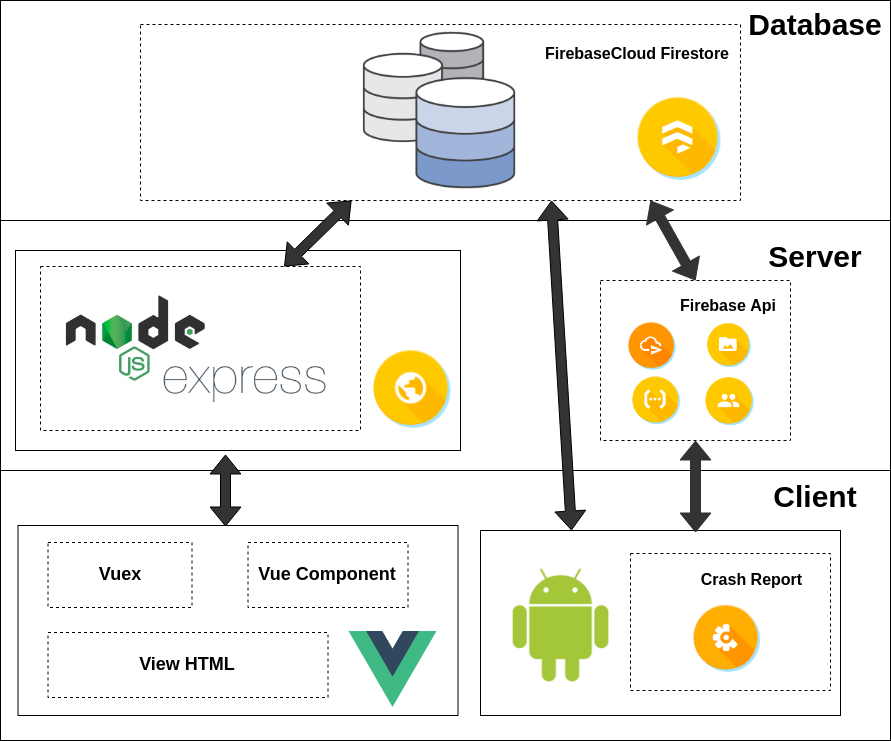
\includegraphics[width=\textwidth]{Figures/3/architecture/architecture}
   		\caption{System architecture ระบบ XX}
   		\label{Fig:architecture}
   	\end{figure}
   
   จากรูปที่ \ref{Fig:architecture} สามารถอธิบายโครงสร้างและเทคโนโลยีของระบบโดยแบ่งเป็น 3 ส่วนหลัก ดังนี้
   \begin{enumerate}
   	\item Database
   	 ระบบใช้บริการฐานข้อมูลแบบ NoSQL ของไฟร์เบสชื่อ Cloud Firestore
	  \item Server
	   กระบวนการทำงานในส่วนของเซิฟเวอร์ (server) แบ่งเป็น 2 ส่วนได้แก่
	   \begin{itemize}
	   	\item ไฟร์เบส Hosting เป็นบริการสำหรับสร้างโฮสต์ (Host) สำหรับเก็บซอร์สโค้ด (source code) และทำการเผยแพร่สำหรับการพัฒนาเว็บไซต์ ซึ่งในที่นี้ใช้ Node.js และ Express ในการพัฒนา
	   	\item ชุดบริการไฟร์เบส Api ใช้สำหรับการทำงานกับบริการต่าง ๆ ของไฟร์เบสบนแฟลตฟอร์มที่แตกต่างกัน เช่น Authentication ใช้สำหรับการจัดการข้อมูลผู้ใช้หรือไฟร์เบส Storage ที่ใช้สำหรับจัดเก็บไฟล์เอกสารและรูปภาพต่าง ๆ เป็นต้น
	   \end{itemize}
	   \item Client
	    แอปพลิเคชันของระบบกองทุนเงินให้กู้ยืมเพื่อการศึกษา คณะวิทยาศาสตร์ มหาวิทยาลัยอุบลราชธานี แบ่งเป็น 2 ส่วนตามการทำงานบนแฟลตฟอร์ม ดังนี้
	    \begin{itemize}
	    	\item เว็บแอปพลิเคชันวัตถุประสงค์ในใช้งานเพื่อรองรับการทำงานของผู้ใช้งานบนบราวเซอร์โดยพัฒนาด้วย Vue.js
	    	\item โมบายแอปพลิเคชันทำงานบนอุปกรณ์พกพา มีการใช้บริการ Crashlytics ของไฟร์เบสในการติดตามข้อผิดพลาดต่าง ๆ ที่เกิดขึ้น
	    \end{itemize}
   \end{enumerate}

\section{System Requirements}
\subsection{Functional Requirements}
	ระบบกองทุนเงินให้กู้ยืมเพื่อการศึกษา คณะวิทยาศาสตร์ มหาวิทยาลัยอุบลราชธานี แบ่งความสามารถของระบบตามประเภทของผู้ใช้งานดังนี้
	\begin{enumerate}
		\item เจ้าหน้าที่
			\begin{itemize}[label={--}]
				\item สามารถทำการเข้าสู่ระบบได้
				\item สามารถสร้างประกาศหรือประชาสัมพันธ์บนเว็บแอปพลิเคชันได้
				\item สามารถกำหนดวันที่และช่วงเวลาในการส่งเอกสารการกู้ยืมของกองทุนเงินให้กู้ยืมเพื่อการศึกษาได้
				\item สามารถตรวจสอบยืนยันความถูกต้องเอกสารกองทุนเงินให้กู้ยืมเพื่อการศึกษาจากนักศึกษาผ่านเว็บแอปพลิเคชันได้
				\item สามารถทำการอัพโหลดฐานข้อมูลนักศึกษากองทุนเงินให้กู้ยืมเพื่อการศึกษาได้
				\item สามารถส่งข้อความเพื่อติดต่อนักศึกษาในระบบได้
				\item สามารถทำการอัพโหลดเอกสารกองทุนเงินให้กู้ยืมเพื่อการศึกษาที่เกี่ยวข้องเข้าสู่ฐานข้อมูลของระบบได้
				\item สามารถสร้างปฏิทินขั้นตอนการดำเนินการกองทุนเงินให้กู้ยืมเพื่อการศึกษาได้
				\item สามารถสร้างรายการคำถามที่พบบ่อยได้
			\end{itemize}
		\item นักศึกษา
			\begin{itemize}[label={--}]
				\item สามารถสมัครสมาชิกและเข้าสู่ระบบได้
				\item สามารถรับข้อมูลข่าวสารประชาสัมพันธ์ได้
				\item สามารถรับข้อมูลแจ้งเตือนเมื่อมีข่าวสารประชาสัมพันธ์ใหม่ ๆ ผ่านโมบายแอปพลิเคชันได้
				\item สามารถดูปฏิทินกำหนดการการดำเนินงานกองทุนเงินให้กู้ยืมเพื่อการศึกษาได้
				\item สามารถส่งภาพสำเนาเอกสารกองทุนเงินให้กู้ยืมเพื่อการศึกษาเพื่อให้พนักงานตรวจสอบได้
				\item สามารถจองวันที่และเวลาในส่งเอกสารกองทุนเงินให้กู้ยืมเพื่อการศึกษาฉบับจริงได้
				\item สามารถดาวน์โหลดเอกสารกองทุนเงินให้กู้ยืมเพื่อการศึกษาจากฐานข้อมูลของระบบได้
				\item สามารถส่งข้อความเพื่อติดต่อสอบถามกับเจ้าหน้าที่กองทุนเงินให้กู้ยืมเพื่อการศึกษาได้
				\item สามารถดูและแก้ไขข้อมูลส่วนตัวได้
				\item สามารถดูรายการคำถามที่พบบ่อยได้		
			\end{itemize}
	\end{enumerate}

\subsection{Non-functional Requirements}
		\begin{enumerate}
		\item เว็บแอปพลิเคชัน
		\begin{itemize}[label={--}]
			\item ใช้โปรโตคอล (Protocol) แบบ HTTPS (Hypertext Transfer Protocol Secure)  ในการสื่อสารที่ช่วยรักษาความสมบูรณ์ถูกต้องของข้อมูลผู้ใช้และเก็บข้อมูลไว้เป็นความลับระหว่างคอมพิวเตอร์ของผู้ใช้กับเว็บไซต์ 
			\item รองรับการใช้งานของผู้ใช้พร้อมกันอย่างน้อย 100 คน
		\end{itemize}
		\item แอนดรอยด์แอปพลิเคชัน
		\begin{itemize}[label={--}]
			\item การสอบถามข้อมูลและการบันทึกข้อมูลปลอดภัยโดยการใช้งาน Cloud FireStore
			\item รองรับการใช้งานของผู้ใช้พร้อมกันอย่างน้อย 100 คน
		\end{itemize}
	\end{enumerate}
	
\section{User Interface Design}
ในการออกแบบ User Interface Design ของระบบกองทุนเงินให้กู้ยืมเพื่อการศึกษา คณะวิทยาศาสตร์ มหาวิทยาลัยอุบลราชธานี ใช้การออกแบบใน 2 ลักษณะ ได้แก่
	\begin{enumerate}
		\item Low-fidelity Wireframes \\ 
		ใช้งาน Low-fidelity Wireframes สำหรับงานที่เน้นความรวดเร็ว สามารถสื่อสารเพื่อเข้าใจถึงการทำงานของระบบนั้น ๆ ได้ ข้อดีคือ ได้ผลตอบรับอย่างรวดเร็ว สะดวกแก่การแก้ไขงาน แต่ข้อเสียคือ อาจจะได้รูปแบบการ Transition ระหว่างหน้านั้นไม่ค่อยสมจริงเท่าไร
			\begin{figure}[H]
				\centering
				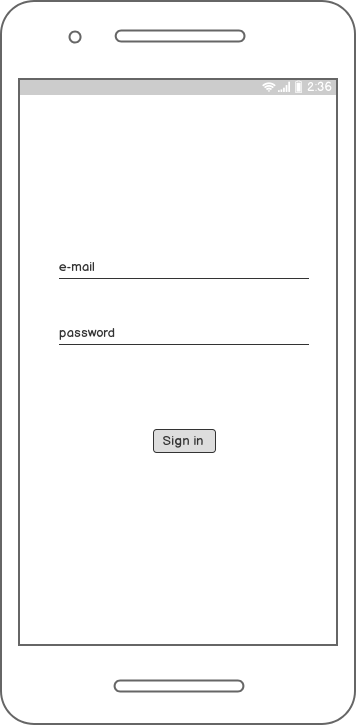
\includegraphics[width=0.3\textwidth]{Figures/3/Wireframe/login}
				\caption{หน้าจอเข้าสู่ระบบ}
				\label{Fig:หน้าจอเข้าสู่ระบบ}
			\end{figure}
			จากภาพที่ \ref{Fig:หน้าจอเข้าสู่ระบบ} แสดงหน้าจอสำหรับให้ผู้ใช้ทำการเข้าสู่ระบบ โดยจำเป็นต้องกรอกข้อมูลอีเมลและรหัสผ่านเพื่อใช้ในการเข้าสู่ระบบ
			\begin{figure}[H]
				\centering
				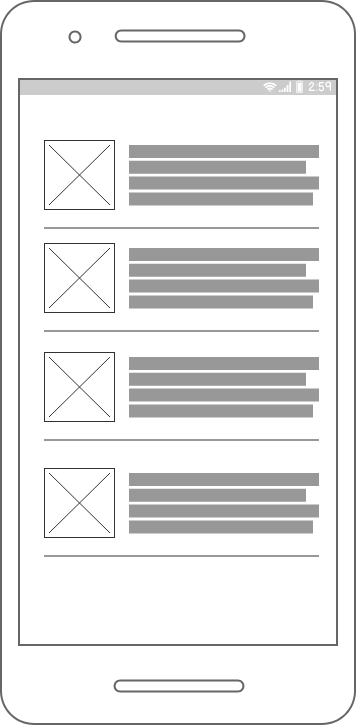
\includegraphics[width=0.3\textwidth]{Figures/3/Wireframe/feed}
				\caption{หน้าจอข่าวสารประชาสัมพันธ์}
				\label{Fig:หน้าจอข่าวสาร}
			\end{figure}
			จากภาพที่ \ref{Fig:หน้าจอข่าวสาร} แสดงหน้าจอข่าวสารหรือประชาสัมพันธ์จากเจ้าหน้าที่หรือผู้ที่เกี่ยวข้องซึ่งแสดงข้อมูลแถวรายการข่าวสารหรือประชาสัมพันธ์
			\begin{figure}[H]
				\centering
				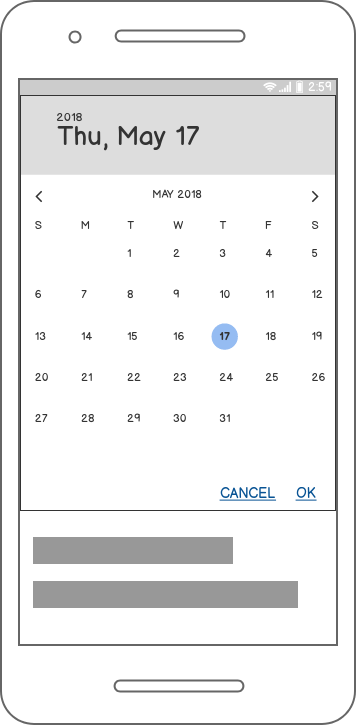
\includegraphics[width=0.3\textwidth]{Figures/3/Wireframe/calendar}
				\caption{หน้าจอปฎิทินกำหนดการ}
				\label{Fig:หน้าจอปฎิธินกำหนดการ}
			\end{figure}
			จากภาพที่ \ref{Fig:หน้าจอปฎิธินกำหนดการ} แสดงหน้าจอปฏิทินกำหนดการการดำเนินการเพื่อให้ผู้ใช้สามารถตรวจสอบกำหนดการวันที่และเวลาในการดำเนินงานของกองทุนโดยหน้าจอมีการแสดงปฏิทินและแถวรายการกำหนดการ

		\item High-fidelity wireframes \\ 
		ใช้งาน High-fidelity wireframes สำหรับการนำเสนอไอเดีย (idea) หรือรูปแบบการ Action ให้แก่ Customer เสมือนงานจริงมากที่สุด ข้อดีคือ สามารถชี้นำการใช้งานจากหน้าหนึ่งไปยังอีกหนึ่งได้ดีด้วยการทำ Motion ระหว่างหน้ารวมทั้งสามารถทำ Interaction กับผู้ใช้งานซึ่งเป็นการสร้างการโต้ตอบการใช้งานกับผู้ใช้ได้ดี
		\begin{itemize}
			\item โมบายแอปพลิเคชัน
			\begin{itemize}
				\item การออกแบบหน้าจอ splash screen 
				\begin{figure}[H]
					\centering
					
\includegraphics[width=0.3\textwidth]{Figures/3/UIMobile/splash_screen}
					\caption{หน้าจอ splash screen}
					\label{Fig:splash_screen}
				\end{figure}
				จากภาพที่ \ref{Fig:splash_screen} แสดงหน้าจอ splash screen ใช้ในการแสดงทุกครั้งที่ผู้ใช้เปิดแอปพลิเคชันโดยวัตถุประสงค์การทำงานของหน้านี้คือเพื่อใช้แสดงขณะที่แอปพลิเคชันทำการประมวลผลข้อมูลบนพื้นหลัง (Background process) เช่น การตรวจสอบสถานะการเข้าสู่ระบบของผู้ใช้คนปัจจุบัน เป็นต้น
				\item การออกแบบหน้าจอเข้าสู่ระบบ
				\begin{figure}[H]
					\centering
					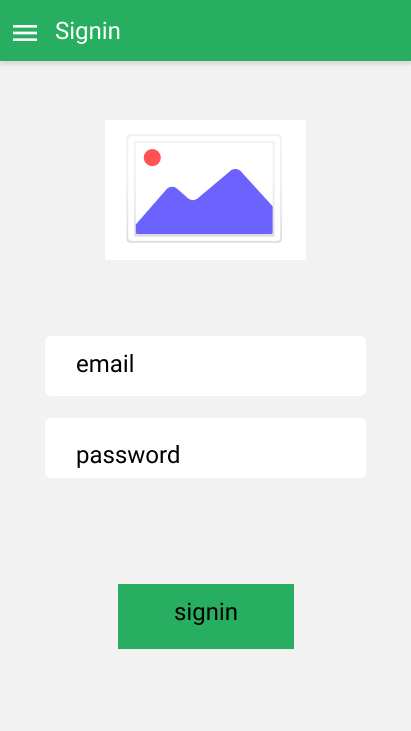
\includegraphics[width=0.3\textwidth]{Figures/3/UIMobile/sign_in}
					\caption{หน้าจอเข้าสู่ระบบ}
					\label{Fig:sign_in}
				\end{figure}
				จากภาพที่ \ref{Fig:sign_in} แสดงหน้าจอสำหรับให้ผู้ใช้ทำการเข้าสู่ระบบเมื่อผู้ใช้ยังไม่ได้ทำการเข้าสู่ระบบ โดยจำเป็นต้องกรอกข้อมูลอีเมลและรหัสผ่านเพื่อใช้ในการเข้าสู่ระบบ ซึ่งการเข้าสู่ระบบจะทำเพียงครั้งเดียวเท่านั้น เมื่อผู้ใช้เปิดการทำงานแอปพลิชันใหม่ในครั้งถัดไประบบจะระบุข้อมูลของผู้ใช้งานอัตโนมัติ
				\item การออกแบบหน้าจอสมัครสมาชิก
				\begin{figure}[H]
					\centering
					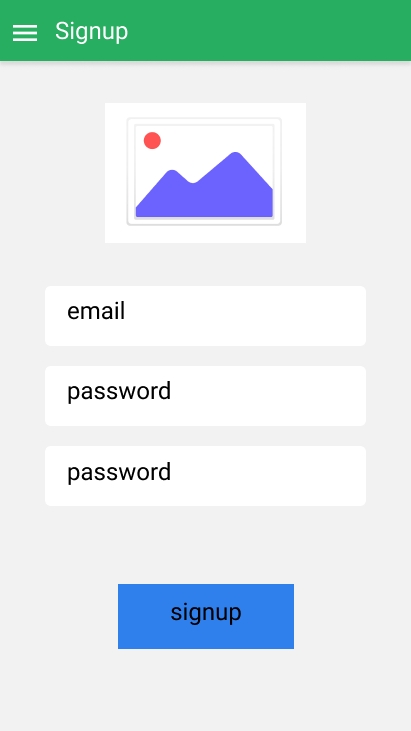
\includegraphics[width=0.3\textwidth]{Figures/3/UIMobile/sign_up}
					\caption{หน้าจอสมัครสมาชิก}
					\label{Fig:sign_up1}
				\end{figure}
				จากภาพที่ \ref{Fig:sign_up1} แสดงหน้าจอสมัครสมาชิก หากผู้ใช้ยังไม่มีบัญชีในระบบผู้ใช้งานสามารถทำการสมัครสมาชิกเพื่อเข้าใช้งานระบบได้จากหน้าสมัครสมาชิก โดยผู้ใช้จำเป็นต้องกรอกข้อมูลอีเมล รหัสผ่านและรหัสนักศึกษาในการสมัครสมาชิก
				\item การออกแบบหน้าจอข่าวสารและประชาสัมพันธ์
				\begin{figure}[H]
					\centering
					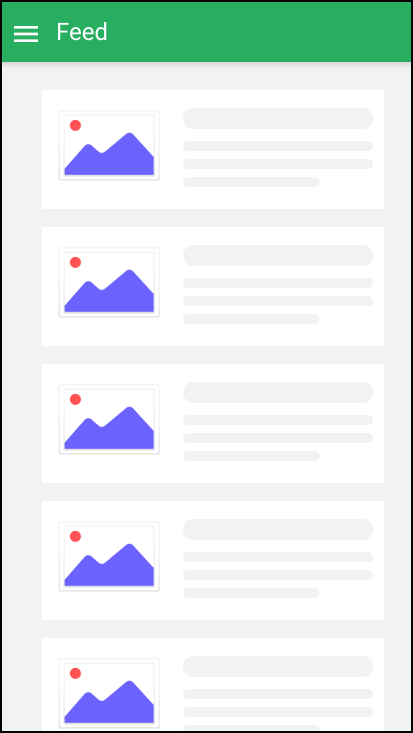
\includegraphics[width=0.3\textwidth]{Figures/3/UIMobile/home_feed}
					\caption{หน้าจอข่าวสารและประชาสัมพันธ์}
					\label{Fig:home_feed}
				\end{figure}
				จากภาพที่ \ref{Fig:home_feed} แสดงหน้าจอข่าวสารหรือประชาสัมพันธ์จากเจ้าหน้าที่หรือผู้ที่เกี่ยวข้อง
				\item การออกแบบหน้าจอเมนูนำทางหลัก 
				\begin{figure}[H]
					\centering
					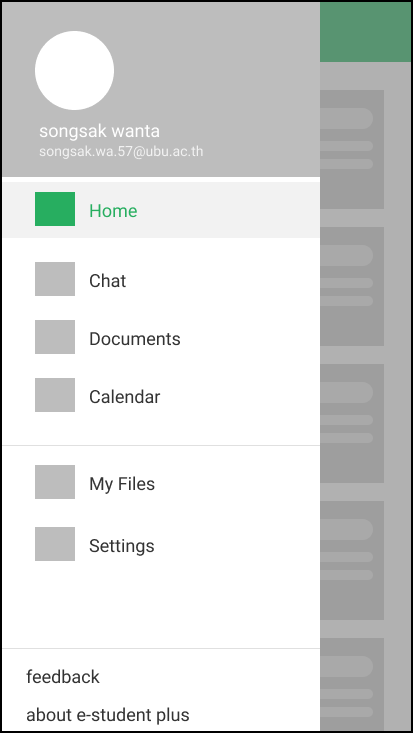
\includegraphics[width=0.3\textwidth]{Figures/3/UIMobile/home_drawer_nav}
					\caption{หน้าจอเมนูนำทางหลัก}
					\label{Fig:home_drawer_nav}
				\end{figure}
				จากภาพที่ \ref{Fig:home_drawer_nav} แสดงเมนูนำทางหลักที่ใช้นำทางผู้ใช้งานไปยังหน้าจออื่นๆ ภายในแอปพลิเคชัน
				\item การออกแบบหน้าจอปฏิทินกำหนดการการดำเนินการ
				\begin{figure}[H]
					\centering
					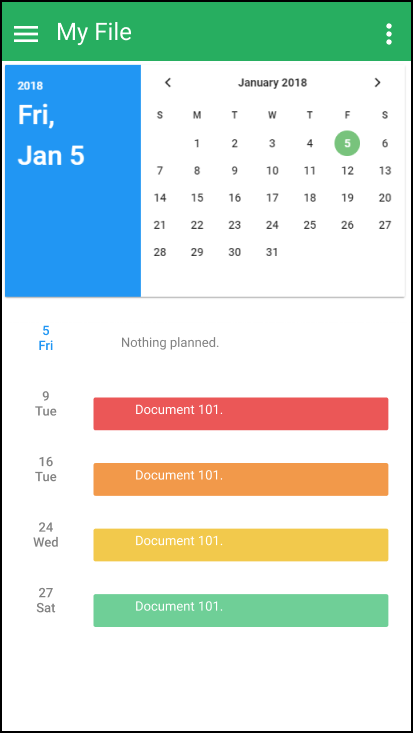
\includegraphics[width=0.3\textwidth]{Figures/3/UIMobile/home_calendar}
					\caption{หน้าจอปฏิทินกำหนดการการดำเนินการ}
					\label{Fig:home_calendar}
				\end{figure}
				จากภาพที่ \ref{Fig:home_calendar} แสดงหน้าจอปฏิทินกำหนดการการดำเนินการเพื่อให้ผู้ใช้สามารถตรวจสอบกำหนดการวันที่และเวลาในการดำเนินงานของกองทุนเงินให้กู้ยืมเพื่อการศึกษา คณะวิทยาศาสตร์ มหาวิทยาลัยอุบลราชธานี
				\item การออกแบบหน้าจอสนทนา
				\begin{figure}[H]
					\centering
					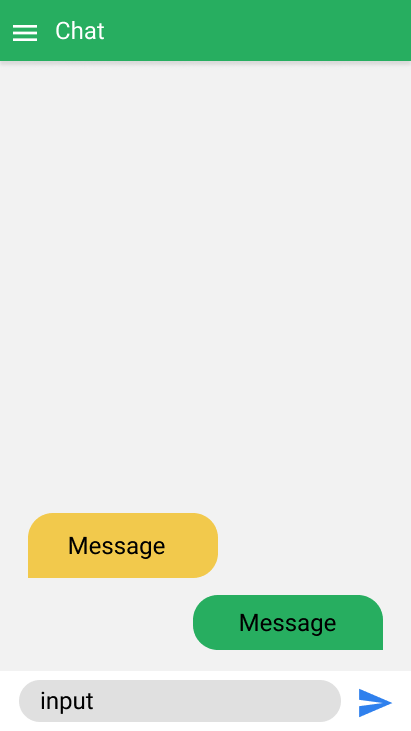
\includegraphics[width=0.3\textwidth]{Figures/3/UIMobile/home_chat}
					\caption{หน้าจอสนทนา}
					\label{Fig:home_chat}
				\end{figure}
				จากภาพที่ \ref{Fig:home_chat} นักศึกษาสามารถส่งข้อความไปยังเจ้าหน้าที่เพื่อติดต่อสอบถามข้อมูลกับทางเจ้าหน้าที่ได้โดยตรง
				\item การออกแบบหน้าจอเอกสารที่เกี่ยวข้อง
				\begin{figure}[H]
					\centering
					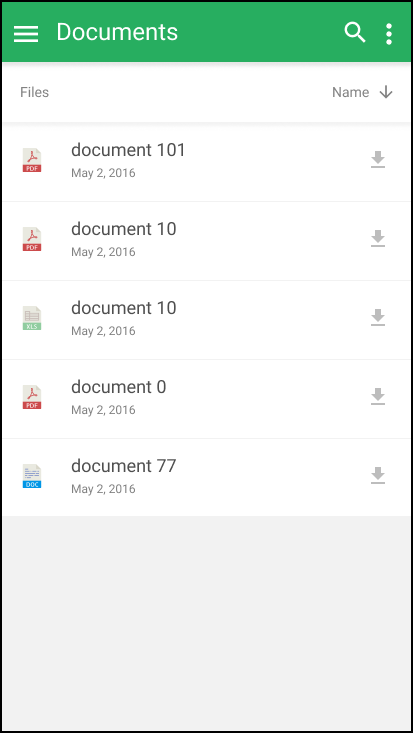
\includegraphics[width=0.3\textwidth]{Figures/3/UIMobile/home_doc}
					\caption{หน้าจอเอกสารที่เกี่ยวข้อง}
					\label{Fig:home_doc}
				\end{figure}
				จากภาพที่ \ref{Fig:home_doc} นักศึกษาสามารถดาวน์โหลดเอกสารที่เกี่ยวข้องกับกองทุนเงินให้กู้ยืมเพื่อการศึกษา คณะวิทยาศาสตร์ มหาวิทยาลัยอุบลราชธานี เช่น ข้อกำหนดและคุณสมบัติของผู้กู้ยืม เป็นต้น ซึ่งเอกสารได้ถูกอัพโหลดไว้โดยเจ้าหน้าที่
				\item การออกแบบหน้าจอจองวันที่และเวลาส่งเอกสาร
				\begin{figure}[H]
					\centering
					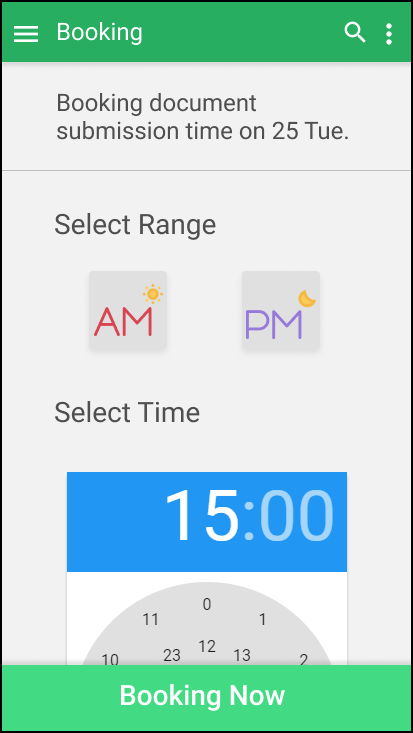
\includegraphics[width=0.3\textwidth]{Figures/3/UIMobile/home_booking}
					\caption{หน้าจอจองวันที่และเวลาส่งเอกสาร}
					\label{Fig:home_booking}
				\end{figure}
				จากภาพที่ \ref{Fig:home_booking}  เมื่อเจ้าหน้าที่ทำการเพิ่มวันที่และช่วงเวลาในการส่งเอกสาร นักศึกษาสามาจองวันที่และเวลาในการส่งเอกสารฉบับจริงของตนได้จากหน้าจอดังกล่าวโดยมีเงื่อนไขคือนักศึกษาผู้ที่จะทำการส่งเอกสารฉบับจริงจำเป็นต้องส่งภาพสำเนาเอกสารผ่านทางระบบเพื่อให้เจ้าหน้าที่ยืนยันความถูกต้องเสียก่อน
			\end{itemize}
			\item เว็บแอปพลิเคชัน
			\begin{itemize}
				\item การออกแบบหน้าจอหลัก
				\begin{figure}[H]
					\centering
					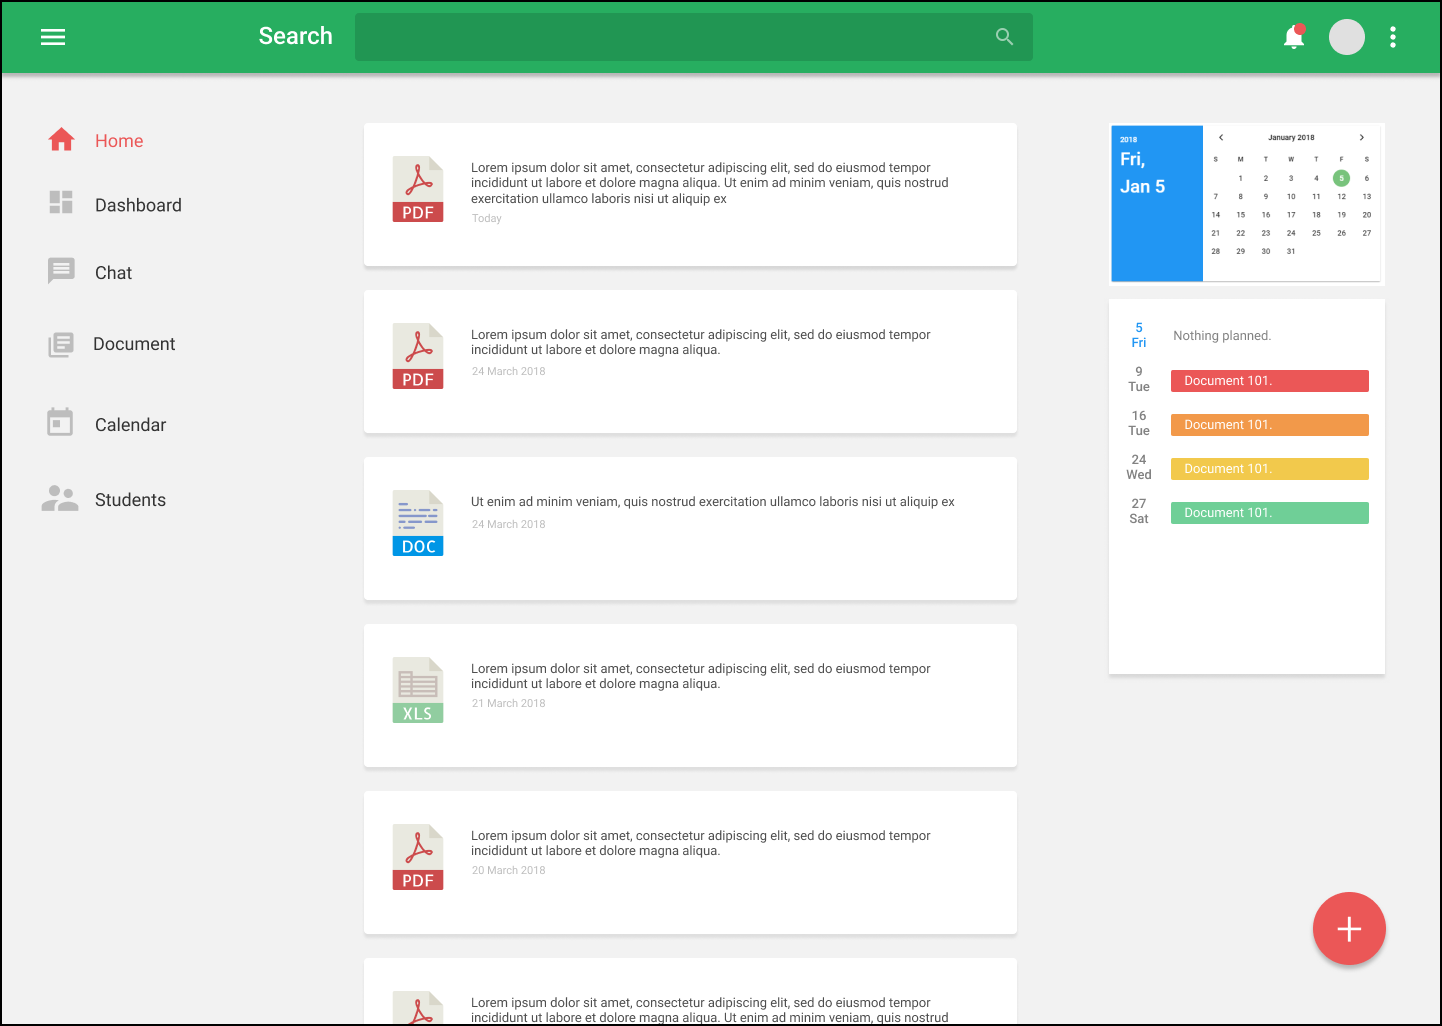
\includegraphics[width=0.8\textwidth]{Figures/3/UIWeb/Home}
					\caption{หน้าจอหลัก}
					\label{Fig:Home}
				\end{figure}
				จากภาพที่ \ref{Fig:Home}  แสดงหน้าจอหลักบนเว็บแอปพลิเคชัน  เพื่ออำนวยความสะดวกต่อเจ้าหน้าที่ ในหน้าหลักได้รวบรวมข้อมูลสรุปและเมนูเข้าถึงด่วนซึ่งแบ่งเป็น 3 ส่วนหลักได้แก่ เมนูนำทาง ข่าวสารประชาสัมพันธ์และปฏิทินกำหนดการ
				\item การออกแบบหน้าจอสนทนา
				\begin{figure}[H]
					\centering
					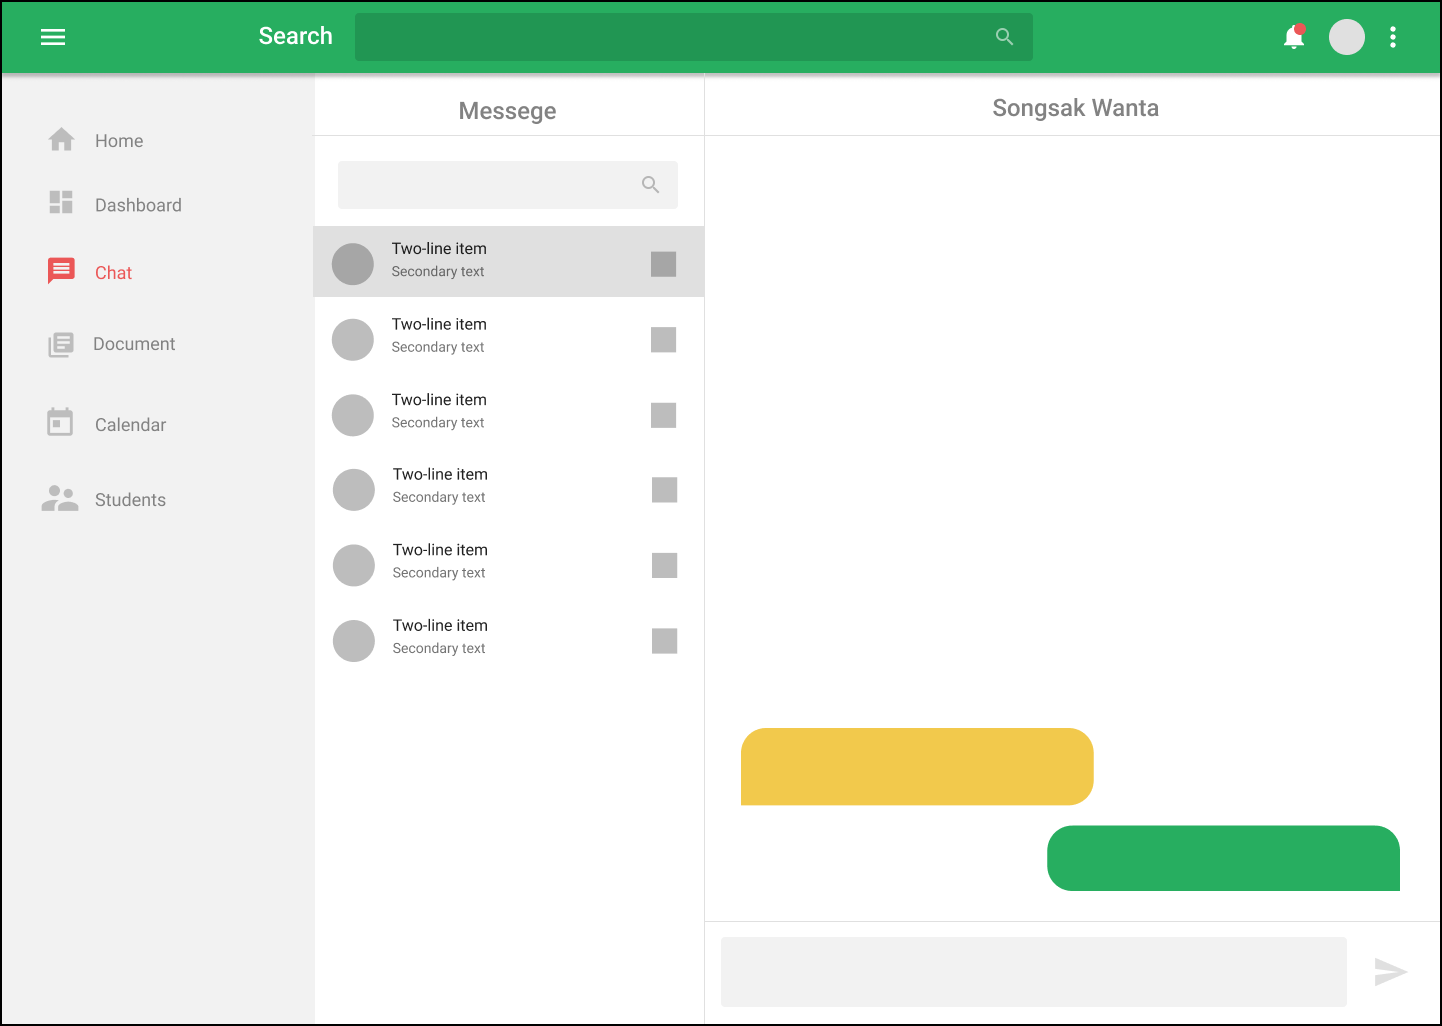
\includegraphics[width=0.8\textwidth]{Figures/3/UIWeb/Chat}
					\caption{หน้าจอสนทนา}
					\label{Fig:Chat}
				\end{figure}
				จากภาพที่ \ref{Fig:Chat}  แสดงหน้าจอสนทนามีการแสดงรายชื่อนักศึกษาและส่วนของห้องสนทนาด้วย
				\item การออกแบบหน้าจออัพโหลดเอกสาร
				\begin{figure}[H]
					\centering
					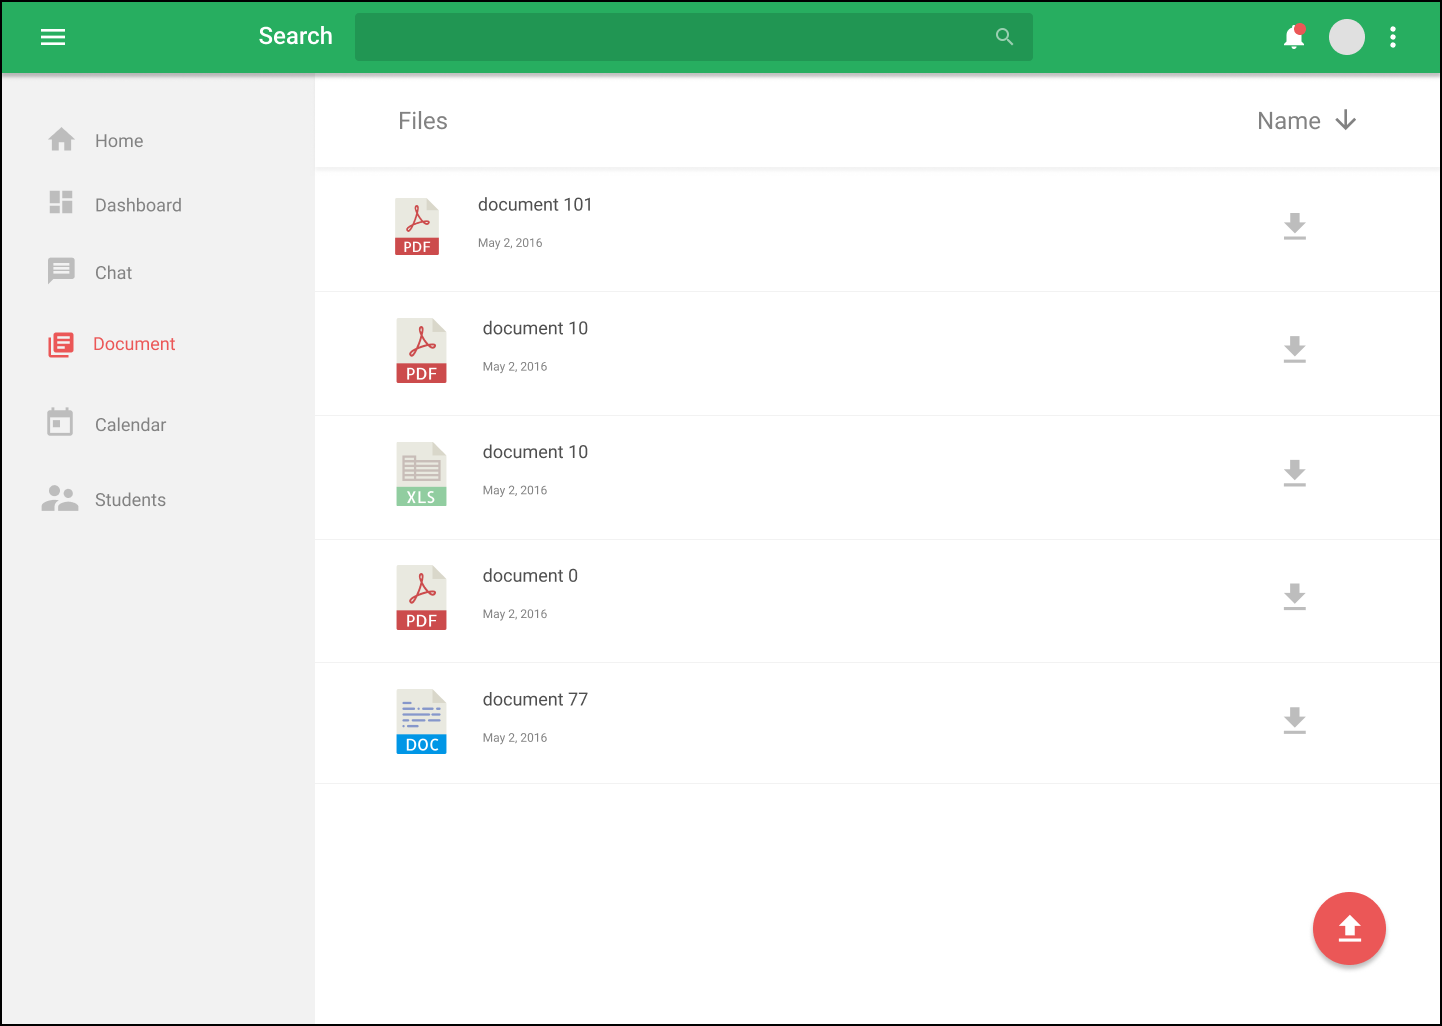
\includegraphics[width=0.8\textwidth]{Figures/3/UIWeb/Doc}
					\caption{หน้าจออัพโหลดเอกสาร}
					\label{Fig:Doc}
				\end{figure}
				จากภาพที่ \ref{Fig:Doc}  แสดงหน้าจออัพโหลดเอกสารที่เกี่ยวข้องกับกองทุนเงินให้กู้ยืมเพื่อการศึกษา คณะวิทยาศาสตร์ มหาวิทยาลัยอุบลราชธานี ทั้งนี้ผู้ที่มีสิทธิ์ในการอัพโหลดเอกสารมีเพียงเจ้าหน้าที่เท่านั้น
				\item การออกแบบหน้าจอเข้าสู่ระบบ
				\begin{figure}[H]
					\centering
					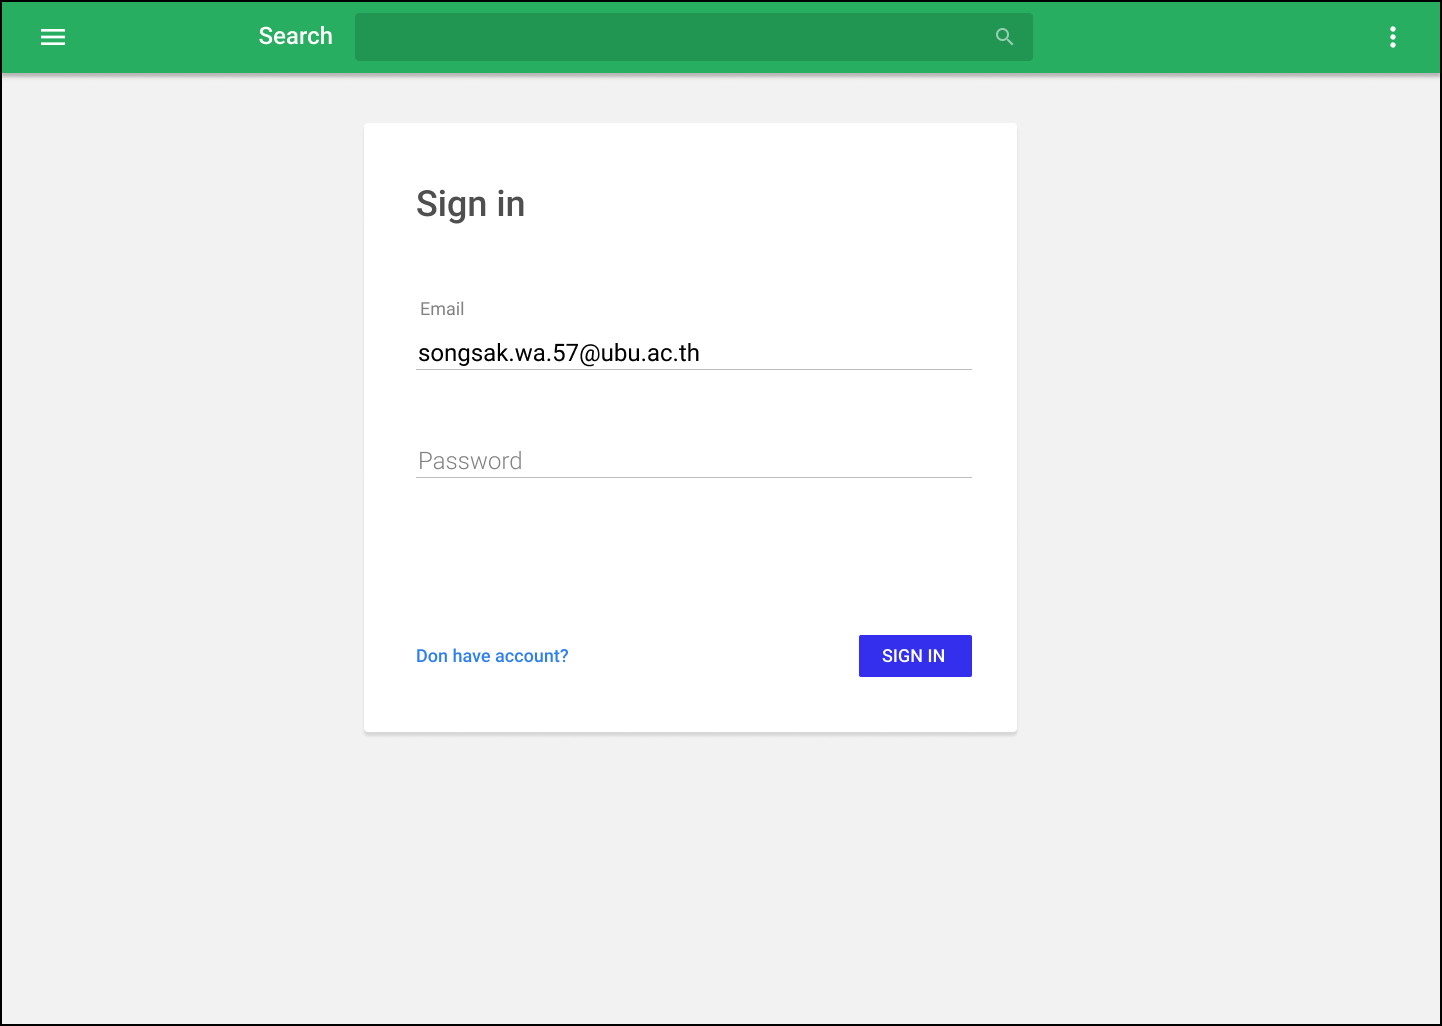
\includegraphics[width=0.8\textwidth]{Figures/3/UIWeb/Login}
					\caption{หน้าจอเข้าสู่ระบบ}
					\label{Fig:Login}
				\end{figure}
				จากภาพที่ \ref{Fig:Login} แสดงหน้าจอการเข้าสู่ระบบของผู้ใช้โดยผู้ใช้จำเป็นต้องกรอกข้อมูลอีเมลและรหัสผ่านเพื่อเข้าใช้งานระบบ
			\end{itemize}
		\end{itemize}
	\end{enumerate}
\newpage

\section{Use Case Diagram}
	Use Case Diagram เป็นแผนผังเพื่อแสดงฟังก์ชันแสดงการทำงานของระบบโดยรวม แสดงส่วนประกอบในระบบและกิจกรรมที่เกิดขึ้นในระบบซึ่งในระบบระบบกองทุนเงินให้กู้ยืมเพื่อการศึกษา คณะวิทยาศาสตร์ มหาวิทยาลัยอุบลราชธานี ผู้ใช้จำเป็นต้องเข้าสู่ระบบเพื่อใช้งานระบบ สัญลักษณ์ที่ใช้ในการเขียน Use Case Diagram แสดงในตารางที่ \ref{tab:use-case2}
	\begin{table}[H]
		\caption{สัญลักษณ์ของ Use case Diagram}
		\label{tab:use-case2}
		\begin{tabular}{|c|p{10cm}|}
		\hline
		\textbf{สัญลักษณ์} & \multicolumn{1}{c|}{\textbf{การใช้งาน}} \\ \hline
		\raisebox{-\totalheight}{Use case}
		& \setstretch{1.5} {Use case คือส่วนย่อยของระบบงาน แทนด้วยวงรีและชื่อของ Use case ภายในวงรี} \\ \hline
		\raisebox{-\totalheight}{
\includegraphics[height=1.5cm]{Figures/table/use-case/2}}
		& \setstretch{1.5} {Actor คือบุคคลหรือระบบงานอื่นที่ใช้งานระบบหรือได้รับประโยชน์จากระบบซึ่งอยู่ภายนอกระบบ แทนด้วยรูปคนและมีชื่อบทบาทการใช้งานระบบ} \\ \hline
		\raisebox{-\totalheight}{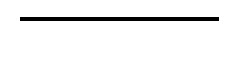
\includegraphics[width=3cm]{Figures/table/use-case/3}}
		& \setstretch{1.5} {เส้นตรงที่แสดงถึงการใช้งาน Use case ของผู้กระทำ} \\ \hline
		\raisebox{-\totalheight}{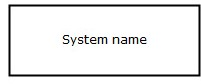
\includegraphics[width=0.3\textwidth]{Figures/table/use-case/4}}
		& \setstretch{1.5} {กรอบสี่เหลี่ยมแสดงถึงขอบเขตของระบบโดยแสดงชื่อระบบภายในหรือด้านบนกรอกสี่เหลี่ยม Use case อยู่ภายในกรอบสี่เหลี่ยม และ actor อยู่ภายนอกกรอบสี่เหลี่ยม} \\ \hline
		\raisebox{-\totalheight}{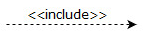
\includegraphics[width=0.3\textwidth]{Figures/table/use-case/5}}
		& \setstretch{1.5} {ความสัมพันธ์แบบ <<includes>> แสดงว่า Use case หนึ่งดำเนินการตามขั้นตอนของ Use case อื่น โดยแทนด้วยสัณลักษณ์ลูกศรเส้นประ ซึ่ง Use case ที่หางลูกศรเรียกใช้งาน Use case ที่หัวลูกศรทุกครั้งที่มีการทำงาน} \\ \hline
		\raisebox{-\totalheight}{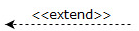
\includegraphics[width=0.3\textwidth]{Figures/table/use-case/6}}
		& \setstretch{1.5} {ความสัมพันธ์แบบ <<extend>> แสดงว่า Use case หนึ่งดำเนินการตามขั้นตอนของ Use case อื่น โดยแทนด้วยสัญลักษณ์ลูกศรเส้นประ ซึ่ง Use case ที่หัวลูกศรเรียกใช้งาน Use case ที่หางลูกศร แต่การใช้งานไม่จำเป็นต้องเกิดขึ้นทุกครั้งขึ้นอยู่กับเงื่อนไขระหว่างการทำงาน} \\ \hline
		\end{tabular}
	\end{table}

	\begin{figure}[H]
		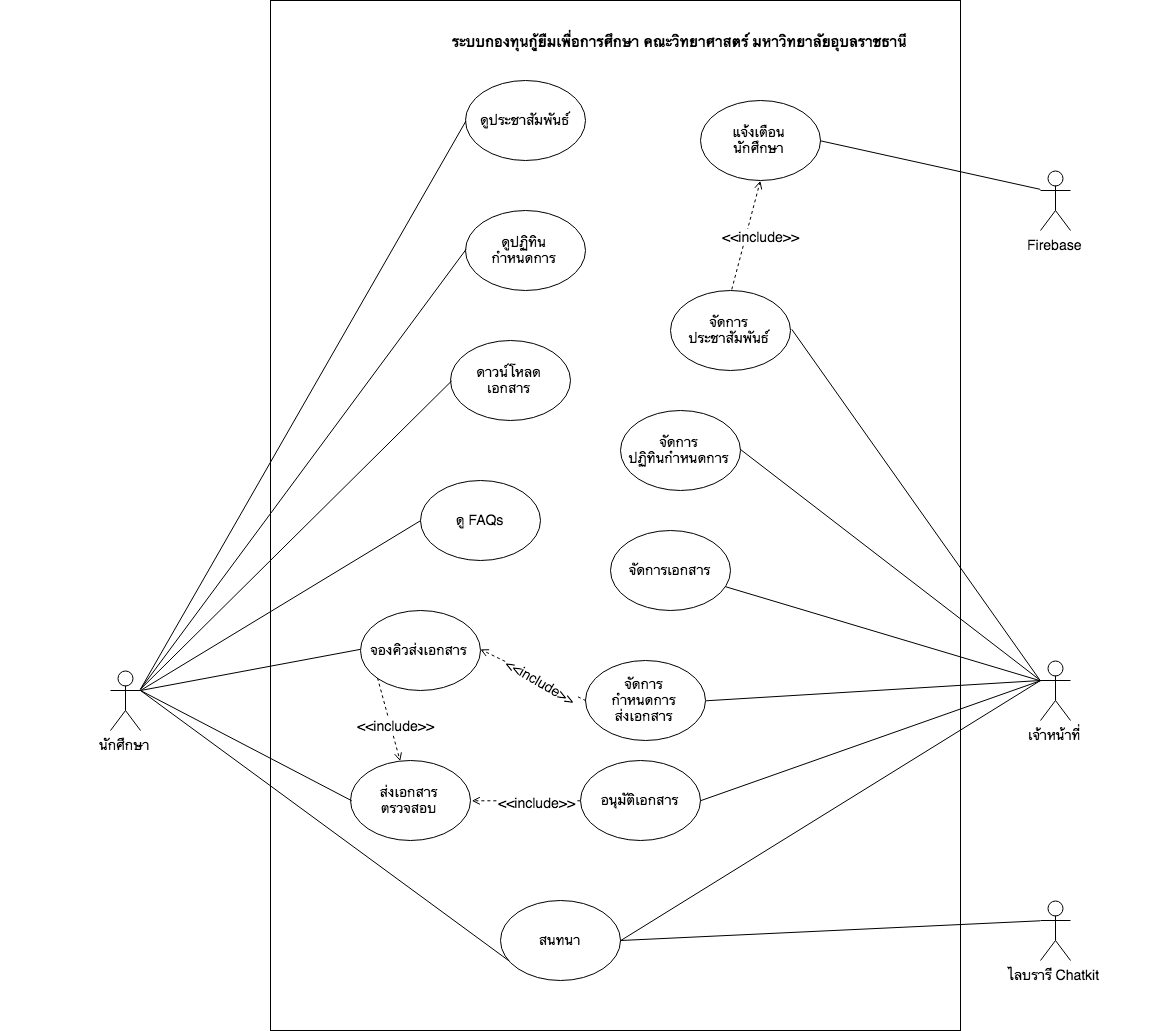
\includegraphics[width=1.2\textwidth]{Figures/3/usecase}
		\caption{Use Case Diagram ของระบบ XX}
		\label{Fig:usecase}
	\end{figure}
	
	\begin{table}[H]
		\centering
		\caption{อธิบาย Use Case หน้าที่ของระบบ ในภาพที่ \ref{Fig:usecase}}
		\label{tab:usecase}
		\resizebox{\totalheight}{!}{\textwidth}{%
			\begin{tabular}{|c|p{10cm}|}
				\hline
				\multicolumn{1}{|c|}{\textbf{Use Case}} & \multicolumn{1}{c|}{\textbf{คำอธิบาย}} \\ \hline
				ดูประชาสัมพันธ์ & นักศึกษาสามารถดูประชาสัมพันธ์ได้โดยไม่จำเป็นต้องทำการเข้าสู่ระบบก่อน \\ \hline
				ดูปฏิทินกำหนดการ & นักศึกษาสามารถเปิดดูปฏิทินวันที่และเวลากำหนดการของกองทุนเงินให้กู้ยืมเพื่อการศึกษา คณะวิทยาศาสตร์วิทยาลัยอุบลราชธานี โดยไม่จำเป็นต้องทำการเข้าสู่ระบบก่อน \\ \hline
				ดาวน์โหลดเอกสาร & นักศึกษาดาวน์โหลดเอกสารที่เกี่ยวข้องกับกองทุนกู้ยีมการศึกษาคณะวิทยาศาสตร์มหาวิทยาลัยอุบลราชธานีได้โดยไม่จำเป็นต้องทำการเข้าสู่ระบบก่อน \\ \hline
				ดู FAQs & หน้าแสดงรายการคำถามที่พบบ่อย \\ \hline
				จองคิวส่งเอกสาร & เมื่อนักศึกษาเข้าสู่ระบบเรียบร้อยแล้วนักศึกษา สามารถจองคิววันที่และเวลาในการส่งเอกสารฉบับจริงหลังจากที่ได้รับการตรวจสอบโดยเจ้าหน้าที่เรียบร้อยแล้ว \\ \hline
				ส่งเอกสารตรวจสอบ & นักศึกษาสามารถส่งเอกสารหน้าที่ตรวจสอบโดยการถ่ายรูปแล้วทำการอัพโหลดเข้าสู่ระบบ เมื่อเจ้าหน้าที่ตรวจสอบเรียบร้อยแล้วจะยืนยันสถานะของเอกสารอีกที \\ \hline
				สนทนา & นักศึกษาสามารถสอบถามข้อมูลของกองทุนเงินให้กู้ยืมเพื่อการศึกษา คณะวิทยาศาสตร์ มหาวิทยาลัยอุบลราชธานี ได้จากช่องสนทนา \\ \hline
				จัดการกำหนดการส่งเอกสาร & ใช้สำหรับเจ้าหน้าที่เพื่อ เพิ่ม แก้ไขหรือลบกำหนดการส่งเอกสารของนักศึกษา \\ \hline
			\end{tabular}%
		}
	\end{table}
		\begin{table}[H]
			\centering
			\caption{อธิบาย Use Case หน้าที่ของระบบ(ต่อ) ในภาพที่ \ref{tab:usecase-15}}
			\label{tab:usecase-15}
			\resizebox{\totalheight}{!}{\textwidth}{%
				\begin{tabular}{|c|p{10cm}|}
					\hline
					\multicolumn{1}{|c|}{\textbf{Use Case}} & \multicolumn{1}{c|}{\textbf{คำอธิบาย}} \\ \hline
					จัดการประชาสัมพันธ์ & ใช้สำหรับเจ้าหน้าที่เพื่อ เพิ่ม แก้ไขหรือลบประชาสัมพันธ์ \\ \hline
					จัดการปฏิทินกำหนดการ & ใช้สำหรับเจ้าหน้าที่เพื่อ เพิ่ม แก้ไขหรือลบกำหนดการการดำเนินการของกองทุน \\ \hline
					จัดการเอกสาร & ใช้สำหรับเจ้าหน้าที่เพื่อ เพิ่ม แก้ไขหรือลบเอกสารที่เกี่ยวข้องของกองทุน \\ \hline
					แจ้งเตือนนักศึกษา & ใช้เพื่อส่งแจ้งเตือนไปยังนักศึกษาเมื่อมีการเพิ่มประชาสัมพันธ์โดยเจ้าหน้าที่ \\ \hline
				\end{tabular}%
			}
		\end{table}
	% Please add the following required packages to your document preamble:
	% \usepackage{graphicx}
	\begin{table}[H]
		\centering
		\caption{Use Case ดูประชาสัมพันธ์}
		\label{tab:usecase}
		\resizebox{\totalheight}{!}{\textwidth}{%
			\begin{tabular}{|p{10cm}|p{10cm}|}
				\hline
				\multicolumn{1}{|c|}{\textbf{Use Case Title : ดูประชาสัมพันธ์}} & \multicolumn{1}{c|}{\textbf{Use case Id : 1 }} \\ \hline
				\multicolumn{2}{|p{\linewidth}|}{Primary Actor : นักศึกษา} \\ \hline
			    \multicolumn{2}{|p{\linewidth}|}{Stakeholder Actor : เจ้าหน้าที่} \\ \hline
			    \multicolumn{2}{|p{\linewidth}|}{Main Flow : นักศึกษาดูประชาสัมพันธ์โดยไม่จำเป็นต้องเข้าสู่ระบบ} \\ \hline
			    \multicolumn{2}{|p{\linewidth}|}{Exceptional Flow ที่ 1 : หากผู้ใช้ไม่เชื่อมต่ออินเทอร์เน็ต จะไม่สามารถดูประชาสัมพันธ์ได้} \\ \hline
			\end{tabular}%
		}
	\end{table}
	\begin{table}[H]
		\centering
		\caption{Use Case ดูปฏิทินกำหนดการ}
		\label{tab:usecase}
		\resizebox{\totalheight}{!}{\columnwidth}{%
			\begin{tabular}{|p{7cm}|p{7cm}|}
				\hline
				\multicolumn{1}{|c|}{\textbf{Use Case Title : ดูปฏิทินกำหนดการ}} & \textbf{Use case Id : 2 } \\ \hline
				\multicolumn{2}{|l|}{Primary Actor : นักศึกษา} \\ \hline
				\multicolumn{2}{|l|}{Stakeholder Actor : เจ้าหน้าที่} \\ \hline
				\multicolumn{2}{|p{\linewidth}|}{Main Flow : นักศึกษาสามารถเปิดดูปฏิทินวันที่และเวลากำหนดการของกองทุนเงินให้กู้ยืมเพื่อการศึกษา  คณะวิทยาศาสตร์ มหาวิทยาลัยอุบลราชธานี ไม่จำเป็นต้องเข้าสู่ระบบ} \\ \hline
				\multicolumn{2}{|p{\linewidth}|}{Exceptional Flow ที่ 1 : หากผู้ใช้ไม่เชื่อมต่ออินเทอร์เน็ต จะไม่สามารถดูปฏิทินกำหนดการได้} \\ \hline
			\end{tabular}%
		}
	\end{table}

	\begin{table}[H]
		\centering
		\caption{Use Case ดาวน์โหลดเอกสาร}
		\label{tab:usecase}
		\resizebox{\totalheight}{!}{\textwidth}{%
			\begin{tabular}{|p{7cm}|p{7cm}|}
				\hline
				\multicolumn{1}{|c|}{\textbf{Use Case Title : ดาวน์โหลดเอกสาร}} & \textbf{Use case Id : 3 } \\ \hline
				\multicolumn{2}{|l|}{Primary Actor : นักศึกษา} \\ \hline
				\multicolumn{2}{|l|}{Stakeholder Actor : เจ้าหน้าที่} \\ \hline
				\multicolumn{2}{|p{\linewidth}|}{Main Flow : นักศึกษาดาวน์โหลดเอกสารที่เกี่ยวข้องกับกองทุนกู้ยีมการศึกษา
				คณะวิทยาศาสตร์มหาวิทยาลัยอุบลราชธานีได้ไม่จำเป็นต้องเข้าสู่ระบบ} \\ \hline
				\multicolumn{2}{|p{\linewidth}|}{Exceptional Flow ที่ 1 : หากผู้ใช้ไม่เชื่อมต่ออินเทอร์เน็ต จะไม่สามารดาวน์โหลดเอกสารที่เกี่ยวข้องกับกองทุนได้} \\ \hline
				\multicolumn{2}{|p{\linewidth}|}{Exceptional Flow ที่ 2 : หากผู้ใช้โมบายแอปพลิเคชันไม่เปิดสิทธิ์การอ่านและเขียนไฟล์บนความจำสำรอง จะไม่สามารถดาวน์โหลดเอกสารที่เกี่ยวข้องกับกองทุนได้} \\ \hline
			\end{tabular}%
		}
		\end{table}
		
		\begin{table}[H]
			\centering
			\caption{Use Case ดู FAQs}
			\label{tab:usecase}
			\resizebox{\totalheight}{!}{\textwidth}{%
				\begin{tabular}{|p{10cm}|p{10cm}|}
					\hline
					\multicolumn{1}{|c|}{\textbf{Use Case Title : ดู FAQs}} & \multicolumn{1}{c|}{\textbf{Use case Id : 4 }} \\ \hline
					\multicolumn{2}{|l|}{Primary Actor : นักศึกษา} \\ \hline
					\multicolumn{2}{|l|}{Stakeholder Actor : เจ้าหน้าที่} \\ \hline
					\multicolumn{2}{|p{\linewidth}|}{Main Flow : ใช้เพื่อแสดงรายการคำถามที่พบบ่อย } \\ \hline
					\multicolumn{2}{|p{\linewidth}|}{Exceptional Flow ที่ 1 : หากผู้ใช้ไม่เชื่อมต่ออินเทอร์เน็ต จะไม่สามารถดูคำถามที่พบบ่อยได้} \\ \hline
				\end{tabular}%
			}
		\end{table}
		
		\begin{table}[H]
			\centering
			\caption{Use Case จองคิวส่งเอกสาร}
			\label{tab:usecase}
			\resizebox{\totalheight}{!}{\textwidth}{%
				\begin{tabular}{|c|p{10cm}|}
					\hline
					\multicolumn{1}{|c|}{\textbf{Use Case Title : จองคิวส่งเอกสาร}} & \multicolumn{1}{c|}{\textbf{Use case Id : 5 }} \\ \hline
					\multicolumn{2}{|l|}{Primary Actor : นักศึกษา} \\ \hline
					\multicolumn{2}{|l|}{Stakeholder Actor : เจ้าหน้าที่} \\ \hline
					\multicolumn{2}{|p{\linewidth}|}{Main Flow :เมื่อนักศึกษาเข้าสู่ระบบเรียบร้อยแล้วนักศึกษา สามารถจองคิววันที่และเวลาในการส่งเอกสารฉบับจริงหลังจากที่ได้รับการตรวจสอบโดยเจ้าหน้าที่เรียบร้อยแล้ว } \\ \hline
					\multicolumn{2}{|p{\linewidth}|}{Exceptional Flow ที่ 1 : หากผู้ใช้ไม่เชื่อมต่ออินเทอร์เน็ต จะไม่สามารถจองคิวส่งเอกสารได้} \\ \hline
				\end{tabular}%
			}
		\end{table}
	
		\begin{table}[H]
			\centering
			\caption{Use Case ส่งเอกสารตรวจสอบ}
			\label{tab:usecase}
			\resizebox{\totalheight}{!}{\textwidth}{%
				\begin{tabular}{|c|p{10cm}|}
					\hline
					\multicolumn{1}{|c|}{\textbf{Use Case Title : ส่งเอกสารตรวจสอบ}} & \multicolumn{1}{c|}{\textbf{Use case Id : 6 }} \\ \hline
					\multicolumn{2}{|l|}{Primary Actor : นักศึกษา} \\ \hline
					\multicolumn{2}{|l|}{Stakeholder Actor : เจ้าหน้าที่} \\ \hline
					\multicolumn{2}{|p{\linewidth}|}{Main Flow : นักศึกษาสามารถส่งเอกสารหน้าที่ตรวจสอบโดยการถ่ายรูปแล้วทำการอัพโหลดเข้าสู่ระบบ เมื่อเจ้าหน้าที่ตรวจสอบเรียบร้อยแล้วจะยืนยันสถานะของเอกสารอีกที } \\ \hline
					\multicolumn{2}{|p{\linewidth}|}{Exceptional Flow ที่ 1 : หากผู้ใช้ไม่เชื่อมต่ออินเทอร์เน็ต จะไม่สามารถส่งเอกสารตรวจสอบได้} \\ \hline
					\multicolumn{2}{|p{\linewidth}|}{Exceptional Flow ที่ 1 : หากผู้ใช้โมบายแอปพลิเคชันไม่เปิดสิทธิ์ใช้งานกล้อง จะไม่สามารถถ่ายภาพเพื่อส่งเอกสารตรวจสอบได้} \\ \hline
				\end{tabular}%
			}
		\end{table}	
		
		\begin{table}[H]
			\centering
			\caption{Use Case สนทนา}
			\label{tab:usecase}
			\resizebox{\totalheight}{!}{\textwidth}{%
				\begin{tabular}{|c|p{10cm}|}
					\hline
					\multicolumn{1}{|c|}{\textbf{Use Case Title : สนทนา}} & \multicolumn{1}{c|}{\textbf{Use case Id : 7 }} \\ \hline
					\multicolumn{2}{|l|}{Primary Actor : นักศึกษา} \\ \hline
					\multicolumn{2}{|l|}{Stakeholder Actor : เจ้าหน้าที่} \\ \hline
					\multicolumn{2}{|p{\linewidth}|}{Main Flow : เมื่อนักศึกษาเข้าสู่ระบบแล้วจะสามารถสอบถามข้อมูลของกองทุนเงินให้กู้ยืมเพื่อการศึกษา คณะวิทยาศาสตร์ มหาวิทยาลัยอุบลราชธานี ได้จากช่องสนทนา} \\ \hline
					\multicolumn{2}{|p{\linewidth}|}{Exceptional Flow ที่ 1 : หากผู้ใช้ไม่เชื่อมต่ออินเทอร์เน็ต จะไม่สามารถสนทนาได้} \\ \hline
				\end{tabular}%
			}
		\end{table}	
%		\begin{table}[H]
%			\centering
%			\caption{Use Case สมัครสมาชิก}
%			\label{tab:usecase}
%			\resizebox{\totalheight}{!}{\textwidth}{%
%				\begin{tabular}{|c|p{10cm}|}
%					\hline
%					\multicolumn{1}{|c|}{\textbf{Use Case Title : สมัครสมาชิก}} & \multicolumn{1}{c|}{\textbf{Use case Id : 8 }} \\ \hline
%					\multicolumn{2}{|l|}{Primary Actor : นักศึกษา} \\ \hline
%					\multicolumn{2}{|l|}{Stakeholder Actor : -} \\ \hline
%					\multicolumn{2}{|p{\linewidth}|}{Main Flow : เมื่อนักศึกษาต้องการใช้งานระบบทั้งหมดของกองทุนจำเป็นต้องเข้าสู่ระบบก่อน หากยังไม่มีบัญชีสามารถสมัครได้โดยต้องกรอกข้อมูลอีเมลและรหัสผ่าน} \\ \hline
%					\multicolumn{2}{|p{\linewidth}|}{Exceptional Flow ที่ 1 : หากผู้ใช้ไม่เชื่อมต่ออินเทอร์เน็ต จะไม่สามารถสมัครสมาชิกได้} \\ \hline
%				\end{tabular}%
%			}
%		\end{table}	
%		 \begin{table}[H]
%		 	\centering
%		 	\caption{Use Case เข้าสู่ระบบ}
%		 	\label{tab:usecase}
%		 	\resizebox{\totalheight}{!}{\textwidth}{%
%		 		\begin{tabular}{|c|p{10cm}|}
%		 			\hline
%		 			\multicolumn{1}{|c|}{\textbf{Use Case Title : เข้าสู่ระบบ}} & \multicolumn{1}{c|}{\textbf{Use case Id : 9 }} \\ \hline
%		 			\multicolumn{2}{|l|}{Primary Actor : นักศึกษา} \\ \hline
%		 			\multicolumn{2}{|l|}{Stakeholder Actor : -} \\ \hline
%		 			\multicolumn{2}{|p{\linewidth}|}{Main Flow : เมื่อนักศึกษาต้องการใช้งานระบบทั้งหมดของกองทุนจำเป็นต้องเข้าสู่ระบบก่อนโดยต้องกรอกข้อมูลอีเมลและรหัสผ่าน} \\ \hline
%		 			\multicolumn{2}{|p{\linewidth}|}{Exceptional Flow ที่ 1 : หากผู้ใช้ไม่เชื่อมต่ออินเทอร์เน็ต จะไม่สามารถเข้าสู่ระบบได้} \\ \hline
%		 		\end{tabular}%
%		 	}
%		 \end{table}	
		  \begin{table}[H]
		  	\centering
		  	\caption{Use Case จัดการกำหนดการส่งเอกสาร}
		  	\label{tab:usecase}
		  	\resizebox{\totalheight}{!}{\textwidth}{%
		  		\begin{tabular}{|c|p{10cm}|}
		  			\hline
		  			\multicolumn{1}{|c|}{\textbf{Use Case Title : จัดการกำหนดการส่งเอกสาร}} & \multicolumn{1}{c|}{\textbf{Use case Id : 10 }} \\ \hline
		  			\multicolumn{2}{|l|}{Primary Actor : เจ้าหน้าที่} \\ \hline
		  			\multicolumn{2}{|l|}{Stakeholder Actor : -} \\ \hline
		  			\multicolumn{2}{|p{\linewidth}|}{Main Flow : เจ้าหน้าที่ เพิ่ม แก้ไขหรือลบกำหนดการส่งเอกสารของนักศึกษา} \\ \hline
		  			\multicolumn{2}{|p{\linewidth}|}{Exceptional Flow ที่ 1 : หากเจ้าหน้าที่ไม่เชื่อมต่ออินเทอร์เน็ต จะไม่สามารถ เพิ่ม แก้ไขหรือลบกำหนดการส่งเอกสารของนักศึกษาได้} \\ \hline
		  		\end{tabular}%
		  	}
		  \end{table}	
		  \begin{table}[H]
			    	\centering
			    	\caption{Use Case จัดการประชาสัมพันธ์}
			    	\label{tab:usecase}
			    	\resizebox{\totalheight}{!}{\textwidth}{%
			    		\begin{tabular}{|c|p{10cm}|}
			    			\hline
			    			\multicolumn{1}{|c|}{\textbf{Use Case Title : จัดการประชาสัมพันธ์}} & \multicolumn{1}{c|}{\textbf{Use case Id : 11 }} \\ \hline
			    			\multicolumn{2}{|l|}{Primary Actor : เจ้าหน้าที่} \\ \hline
			    			\multicolumn{2}{|l|}{Stakeholder Actor : -} \\ \hline
			    			\multicolumn{2}{|p{\linewidth}|}{Main Flow : เจ้าหน้าที่ เพิ่ม แก้ไขหรือลบปฏิทินกำหนดการในระบบได้} \\ \hline
			    			\multicolumn{2}{|p{\linewidth}|}{Exceptional Flow ที่ 1 : หากเจ้าหน้าที่ไม่เชื่อมต่ออินเทอร์เน็ต จะไม่สามารถ เพิ่ม แก้ไขหรือลบปฏิทินกำหนดการได้} \\ \hline
			    		\end{tabular}%
			    	}
		  \end{table}	
		    \begin{table}[H]
		    	\centering
		    	\caption{Use Case จัดการปฏิทินกำหนดการ}
		    	\label{tab:usecase}
		    	\resizebox{\totalheight}{!}{\textwidth}{%
		    		\begin{tabular}{|c|p{10cm}|}
		    			\hline
		    			\multicolumn{1}{|c|}{\textbf{Use Case Title : จัดการปฏิทินกำหนดการ}} & \multicolumn{1}{c|}{\textbf{Use case Id : 12 }} \\ \hline
		    			\multicolumn{2}{|l|}{Primary Actor : เจ้าหน้าที่} \\ \hline
		    			\multicolumn{2}{|l|}{Stakeholder Actor : -} \\ \hline
		    			\multicolumn{2}{|p{\linewidth}|}{Main Flow : เจ้าหน้าที่ เพิ่ม แก้ไขหรือลบปฏิทินกำหนดการได้} \\ \hline
		    			\multicolumn{2}{|p{\linewidth}|}{Exceptional Flow ที่ 1 : หากเจ้าหน้าที่ไม่เชื่อมต่ออินเทอร์เน็ต จะไม่สามารถ เพิ่ม แก้ไขหรือลบปฏิทินกำหนดการได้} \\ \hline
		    		\end{tabular}%
		    	}
		    \end{table}	
		   \begin{table}[H]
		   	\centering
		   	\caption{Use Case จัดการเอกสาร}
		   	\label{tab:usecase}
		   	\resizebox{\totalheight}{!}{\textwidth}{%
		   		\begin{tabular}{|c|p{10cm}|}
		   			\hline
		   			\multicolumn{1}{|c|}{\textbf{Use Case Title : จัดการเอกสาร}} & \multicolumn{1}{c|}{\textbf{Use case Id : 13 }} \\ \hline
		   			\multicolumn{2}{|l|}{Primary Actor : เจ้าหน้าที่} \\ \hline
		   			\multicolumn{2}{|l|}{Stakeholder Actor : -} \\ \hline
		   			\multicolumn{2}{|p{\linewidth}|}{Main Flow : เจ้าหน้าที่ เพิ่ม แก้ไขหรือลบเอกสารที่เกี่ยวข้องกับกองทุนได้} \\ \hline
		   			\multicolumn{2}{|p{\linewidth}|}{Exceptional Flow ที่ 1 : หากเจ้าหน้าที่ไม่เชื่อมต่ออินเทอร์เน็ต จะไม่สามารถ เพิ่ม แก้ไขหรือลบเอกสารที่เกี่ยวข้องกับกองทุนได้} \\ \hline
		   		\end{tabular}%
		   	}
		   \end{table}	
			  \begin{table}[H]
			  	\centering
			  	\caption{Use Case แจ้งเตือนนักศึกษา}
			  	\label{tab:usecase}
			  	\resizebox{\totalheight}{!}{\textwidth}{%
			  		\begin{tabular}{|c|p{10cm}|}
			  			\hline
			  			\multicolumn{1}{|c|}{\textbf{Use Case Title : แจ้งเตือนนักศึกษา}} & \multicolumn{1}{c|}{\textbf{Use case Id : 14 }} \\ \hline
			  			\multicolumn{2}{|l|}{Primary Actor : เจ้าหน้าที่} \\ \hline
			  			\multicolumn{2}{|l|}{Stakeholder Actor : -} \\ \hline
			  			\multicolumn{2}{|p{\linewidth}|}{Main Flow : แจ้งเตือนไปยังนักศึกษาเมื่อมีการเพิ่มประชาสัมพันธ์โดยเจ้าหน้าที่} \\ \hline
			  			\multicolumn{2}{|p{\linewidth}|}{Exceptional Flow ที่ 1 : หากนักศึกษาที่ไม่เชื่อมต่ออินเทอร์เน็ต จะไม่สามารถรับแจ้งเตือนเมื่อมีการเพิ่มประชาสัมพันธ์โดยเจ้าหน้าที่} \\ \hline
			  		\end{tabular}%
			  	}
			  \end{table}	
\newpage

\section{Class Diagram}
	Class Diagram คือแผนภาพที่ใช้แสดงคลาสและความสัมพันธ์ในแบบต่างๆ ระหว่างคลาส สัญลักษณ์ที่ใช้ในการเขียน Class Diagram แสดงในตารางที่ \ref{tab:class2} 
	\begin{center}
	\begin{table}[H]
		\centering
		\caption{สัญลักษณ์ของ Class Diagram}
		\label{tab:class2}
		\begin{tabular}{|c|p{10cm}|}
			\hline
			\textbf{สัญลักษณ์} & \multicolumn{1}{c|}{\textbf{การใช้งาน}} \\ \hline
			\raisebox{-\totalheight}{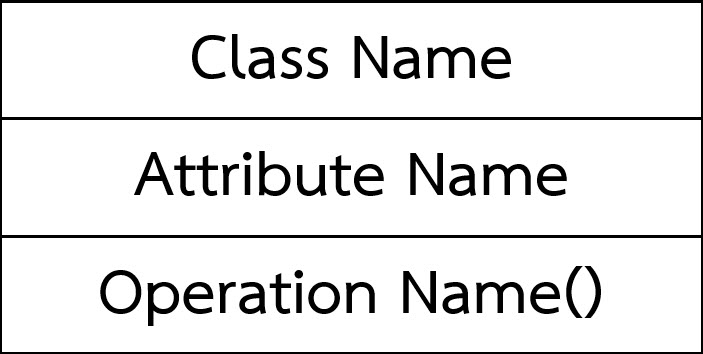
\includegraphics[width=0.3\textwidth]{Figures/table/class/11}}
			& \setstretch{1.5} {คลาส สัญลักษณ์แทนด้วยสี่เหลี่ยมแบ่งเป็น 3 ส่วน 
				ส่วนบน เป็นชื่อของ class ส่วนกลาง เป็นชื่อ Attribute และส่วนล่างเป็น Operation Name หรือ Method ใช้สำหรับเขียนฟังก์ชันในการทำงานของคลาสนั้น ๆ
				ชนิดของ Visibility ของ Method และ Attribute
				แบ่งเป็น 3 ชนิด ได้แก่
				\begin{enumerate}
					\item Public แทนสัญลักษณ์ด้วยเครื่องหมายบวก (+)
					\item Private แทนสัญลักษณ์ด้วยเครื่องหมายลบ (-)
					\item Protected แทนสัญลักษณ์ด้วยเครื่องหมายชาร์ป (#)
				\end{enumerate}
			} \\ \hline
			\raisebox{-\totalheight}{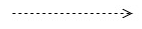
\includegraphics[width=0.3\textwidth]{Figures/table/class/1}}
			& \setstretch{1.5} {Dependency Relationship หมายความว่า คลาสที่อยู่ฝั่งต้นลูกศรสามารถเรียกใช้คลาสที่อยู่ฝั่งหัวลูกศร}
			\\ \hline
			\raisebox{-\totalheight}{
\includegraphics[width=0.35\textwidth]{Figures/3/Class/aggre}}
			& \setstretch{1.5} {Composition Relationship เป็นความสัมพันธ์ระหว่างออบเจ็กต์หรือคลาสแบบขึ้นต่อกันและมีความเกี่ยวข้องกันเสมอ} \\ \hline
			\raisebox{-\totalheight}{
\includegraphics[width=0.3\textwidth]{Figures/3/Class/implement}}
			& \setstretch{1.5} {Realization Relationship เป็นความสัมพันธ์ระหว่าง Object หรือ Class ในลักษณะของการสืบทอดคุณสมบัติจาก Class หนึ่ง (Super class) ไปยังอีก Class หนึ่ง (Subclass)} \\ \hline
			\raisebox{-\totalheight}{
\includegraphics[width=50,height=50]{Figures/table/class/connector}}
			& \setstretch{1.5} {Connector เป็นสัญลักษณ์แทนด้วยรูปห้าเหลี่ยมและมีชื่ออยู่ตรงกลาง จะสร้างสัญลักษณ์นี้ไว้เมื่อต้องการเชื่อมต่อคลาสที่อยู่คนละหน้า} \\ \hline
		\end{tabular}
	\end{table}
	\end{center}

\newpage
  %IMAGE of class
	Class Diagram แสดงความสัมพันธ์ในรูปแบบต่างๆ ระหว่างคลาสของแอปพลิเคชันระบบกองทุนเงินให้กู้ยืมเพื่อการศึกษา คณะวิทยาศาสตร์ มหาวิทยาลัยอุบลราชธานี อธิบายได้ตามภาพที่ \ref{Fig:MainActivity20C} ดังต่อไปนี้
	\begin{figure}[H]
		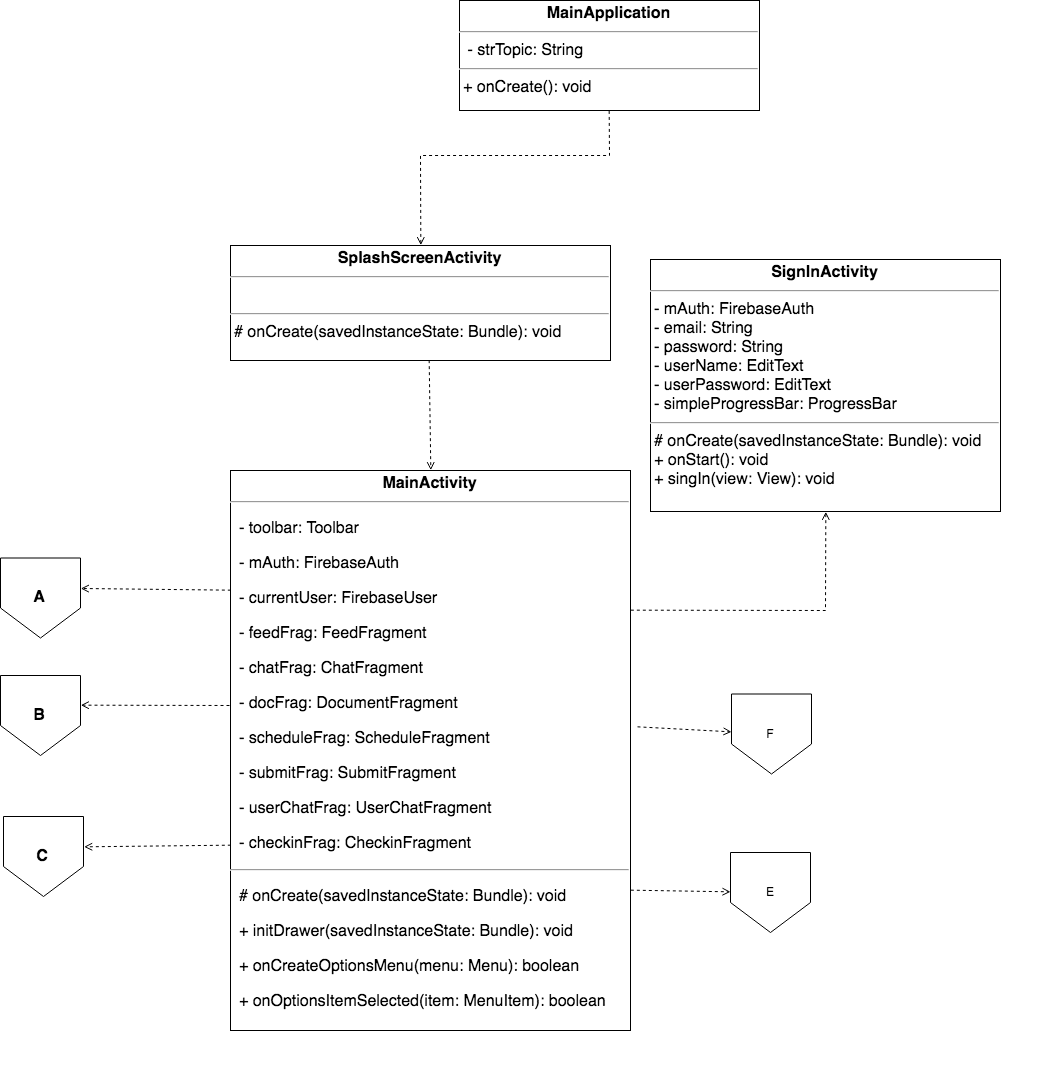
\includegraphics[width=1.0\columnwidth]{Figures/3/Class/MainActivity}
		\caption{Class Diagram ของแอปพลิเคชันระบบ XX}
		\label{Fig:MainActivity20C}
	\end{figure}
	\begin{figure}[H]
		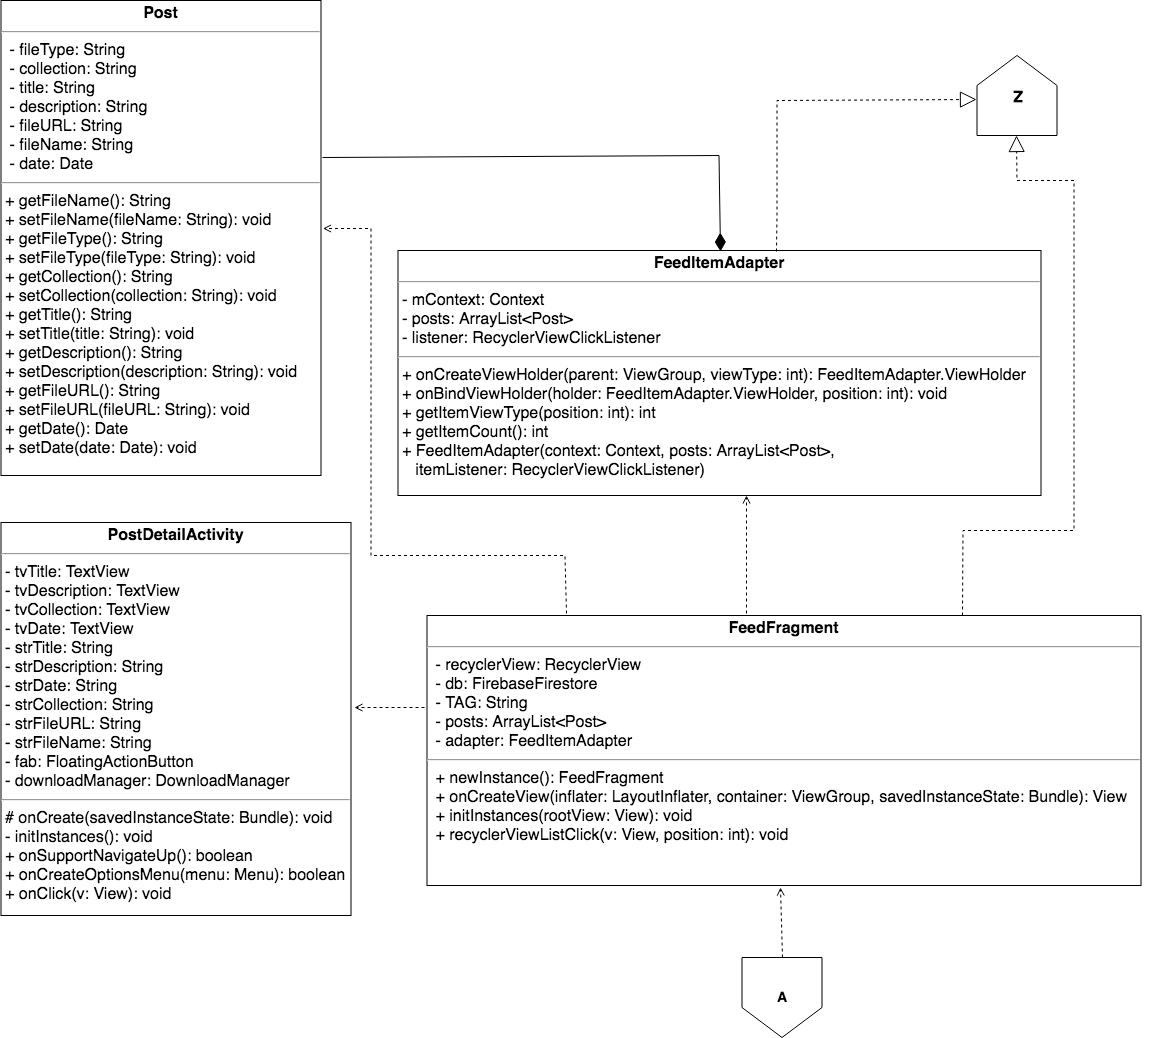
\includegraphics[width=1.0\columnwidth]{Figures/3/Class/Feed}
		\caption{Class Diagram ของแอปพลิเคชันระบบ XX}
		\label{Fig:FeedC}
	\end{figure}
\begin{sidewaysfigure}
	\begin{figure}[H]
		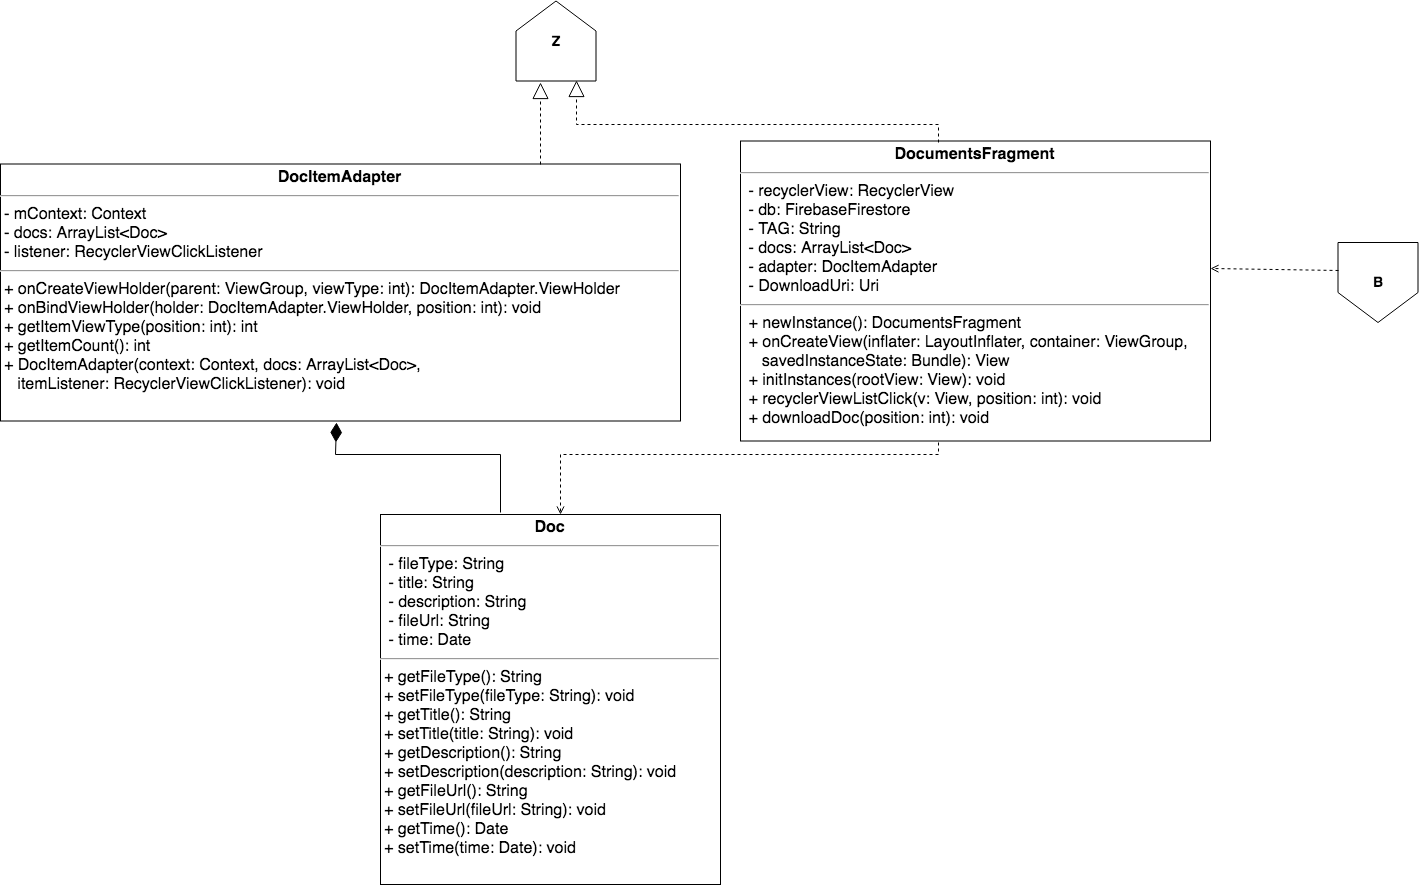
\includegraphics[width=1.0\columnwidth]{Figures/3/Class/Doc}
		\caption{Class Diagram ของแอปพลิเคชันระบบ XX}
		\label{Fig:DocC}
	\end{figure}
\end{sidewaysfigure}
	\begin{figure}[H]
		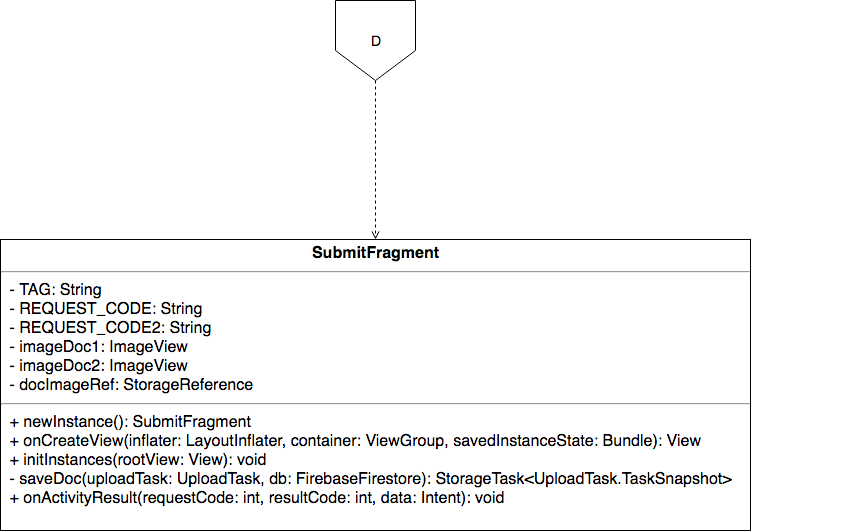
\includegraphics[width=\columnwidth]{Figures/3/Class/Submit}
		\caption{Class Diagram ของแอปพลิเคชันระบบ XX}
		\label{Fig:SubmitC}
	\end{figure}
	\begin{figure}[H]
		
\includegraphics[width=1.0\columnwidth]{Figures/3/Class/UserChat}
		\caption{Class Diagram ของแอปพลิเคชันระบบ XX}
		\label{Fig:UserChatC}
	\end{figure}

	% TABLE of class
\newpage	
	จากรูปภาพที่ \ref{Fig:MainActivity20C} สามารถอธิบายแผนภาพ Class Diagram ได้ดังนี้
	\begin{table}[H]
		\centering
		\caption{อธิบาย Class Diagram ของคลาสพื้นฐานของระบบ}
		\label{tab:class}
		\begin{tabular}{|c|p{10cm}|}
			\hline
			\textbf{Class Diagram} & \multicolumn{1}{c|}{\textbf{คำอธิบาย}} \\ \hline
			\raisebox{-\totalheight}{MainApplication}
			& \setstretch{1.5} {คลาส MainApplication จะถูกเรียกใช้งานทุกครั้งเมื่อผู้ใช้เปิดแอปพลิเคชัน โดยวัตถุประสงค์การทำงานของคลาสนี้คือ เพื่อใช้จัดการทรัพยากรที่จำเป็นสำหรับการใช้งานในคลาสอื่น ๆ } \\ \hline
			\raisebox{-\totalheight}{SplashScreenActivity}
			& \setstretch{1.5} {คลาส SplashScreenActivity จะถูกเรียกใช้งานทุกครั้งเมื่อผู้ใช้เปิดแอปพลิเคชัน โดยวัตถุประสงค์การทำงานของคลาสคือ เพื่อใช้ตรวจสอบสถานะการเข้าสู่ระบบของผู้ใช้} \\ \hline
			\raisebox{-\totalheight}{MainActivity}
			& \setstretch{1.5} {คลาส MainActivity เป็นคลาสหลักที่ใช้ในการทำงานของแอปพลิเคชันโดยการทำงานของคลาสนี้เน้นไปที่การสร้าง Fragment เพื่อใช้แสดงข้อมูลต่าง ๆ โดยองค์ประกอบการทำงานของคลาสนี้ประกอบบไปด้วยสองส่วนหลักๆ ได้แก่ เมนูนำทาง Drawer และ Fragment Container} \\ \hline
			\raisebox{-\totalheight}{SignInActivity}
			& \setstretch{1.5} {คลาส SignInActivity เป็นคลาสที่ใช้เพื่อให้สมาชิกที่ได้ลงทะเบียนกับระบบเข้าสู่ระบบเพื่อใช้งานบริการต่าง ๆ จากระบบ} \\ \hline
	\end{tabular}
\end{table}

\newpage
จากรูปภาพที่ \ref{Fig:FeedC} สามารถอธิบายแผนภาพ Class Diagram ได้ดังนี้
\begin{table}[H]
	\centering
	\caption{อธิบาย Class Diagram ของส่วนของการแสดงข่าวสาร}
	\label{tab:class}
	\begin{tabular}{|c|p{10cm}|}
		\hline
		\textbf{Class Diagram} & \multicolumn{1}{c|}{\textbf{คำอธิบาย}} \\ \hline
		\raisebox{-\totalheight}{FeedFragment}
		& \setstretch{1.5} {คลาส FeedFragment เป็นคลาสหลักที่ใช้ในการแสดงข้อมูลข่าวสาร มีการทำงานหลักคือสืบค้นฐานข้อมูลจากไฟร์เบสเพื่อนำมาแสดง} \\ \hline
		\raisebox{-\totalheight}{FeedItemAdapter}
		& \setstretch{1.5} {คลาส FeedItemAdapter เป็นคลาสที่มีหน้าที่ในการแปลงชุดข้อมูลที่ได้จากคลาส FeedFragment แล้วคืนค่ากลับเป็นลิสต์รายการของชุดข้อมูลนั้น ๆ} \\ \hline
		\raisebox{-\totalheight}{Post}
		& \setstretch{1.5} {คลาส Post เป็นคลาสโมเดลที่กำหนดค่าต่างๆที่จำเป็นสำหรับใช้ในการสร้างลิสต์รายการของคลาส FeedItemAdapter} \\ \hline
		\raisebox{-\totalheight}{PostDetailActivity}
		& \setstretch{1.5} {คลาส PostDetailActivity เป็นคลาสที่มีหน้าที่ในการแสดงข้อมูลรายละเอียดของข่าวสารแต่ละแถวที่ได้รับจากหน้า FeedFragment ที่จะส่งข้อมูลเมื่อผู้ใช้กดที่แถวรายการข่าวสาร} \\ \hline
		\raisebox{-\totalheight}{RecyclerViewClickListener}
		& \setstretch{1.5} {คลาส RecyclerViewClickListener เป็นคลาสอินเทอร์เฟส(Interface)ที่ใช้ในการสร้างแม่แบบเมื่อคลาสใด ๆ ต้องการใช้งานสำหรับการรับค่าเมื่อผู้ใช้กดแถวในลิสต์รายการ คลาสลูกที่ทำการสืบทอดคุณสมบัติจะสามารถรับข้อมูลตำแหน่งแถวที่ผู้ใช้กดบนลิสต์รายการได้} \\ \hline
	\end{tabular}
\end{table}

\newpage
จากรูปภาพที่ \ref{Fig:DocC} สามารถอธิบายแผนภาพ Class Diagram ได้ดังนี้
\begin{table}[H]
	\centering
	\caption{อธิบาย Class Diagram ของส่วนของการแสดงรายการเอกสารในระบบ}
	\label{tab:class}
	\begin{tabular}{|c|p{10cm}|}
		\hline
		\textbf{Class Diagram} & \multicolumn{1}{c|}{\textbf{คำอธิบาย}} \\ \hline
		\raisebox{-\totalheight}{DocumentsFragment}
		& \setstretch{1.5} {คลาส DocumentsFragment เป็นคลาสที่ใช้ในการแสดงข้อมูลเอกสารที่ถูกอัพโหลดเข้าสู่ระบบโดยเจ้าหน้าที่ซึ่งจะถูกแสดงเป็นลิสต์รายการ} \\ \hline
		\raisebox{-\totalheight}{DocItemAdapter}
		& \setstretch{1.5} {คลาส DocItemAdapter เป็นคลาสที่มีหน้าที่ในการแปลงชุดข้อมูลที่ได้รับจากคลาส DocumentsFragment เป็นลิสต์รายการแล้วคืนกลับไปยังคลาส DocumentsFragment} \\ \hline
		\raisebox{-\totalheight}{Doc}
		& \setstretch{1.5} {คลาส Doc เป็นคลาสโมเดลที่กำหนดค่าต่าง ๆ ที่จำเป็นสำหรับใช้ในการสร้างลิสต์รายการของคลาส DocItemAdapter} \\ \hline
		\raisebox{-\totalheight}{RecyclerViewClickListener}
		& \setstretch{1.5} {คลาส RecyclerViewClickListener เป็นคลาสอินเทอร์เฟสที่ใช้ในการสร้างแม่แบบเมื่อคลาสใด ๆ ต้องการใช้งานสำหรับการรับค่าเมื่อผู้ใช้กดแถวในลิสต์รายการ คลาสลูกที่ทำการสืบทอดคุณสมบัติจะสามารถรับข้อมูลตำแหน่งแถวที่ผู้ใช้กดบนลิสต์รายการได้} \\ \hline
	\end{tabular}
\end{table}

\newpage
จากรูปภาพที่ \ref{Fig:SubmitC} สามารถอธิบายแผนภาพ Class Diagram ได้ดังนี้
\begin{table}[H]
	\centering
	\caption{อธิบาย Class Diagram ของส่วนของการส่งสำเนาเอกสาร}
	\label{tab:class}
	\begin{tabular}{|c|p{10cm}|}
		\hline
		\textbf{Class Diagram} & \multicolumn{1}{c|}{\textbf{คำอธิบาย}} \\ \hline
		\raisebox{-\totalheight}{SubmitFragment}
		& \setstretch{1.5} {คลาส SubmitFragment เป็นคลาสที่ใช้ในการแสดงหน้าจอส่งสำเนาเอกสาร โดยมีการดำเนินการภายในคลาสหลัก ๆ ได้แก่ การถ่ายภาพ แปลงภาพและบันทึกภาพเข้าสู่ระบบ} \\ \hline
	\end{tabular}
\end{table}

จากรูปภาพที่ \ref{Fig:UserChatC} สามารถอธิบายแผนภาพ Class Diagram ได้ดังนี้
\begin{table}[H]
	\centering
	\caption{อธิบาย Class Diagram ของส่วนของการสนทนา}
	\label{tab:class}
	\begin{tabular}{|c|p{10cm}|}
		\hline
		\textbf{Class Diagram} & \multicolumn{1}{c|}{\textbf{คำอธิบาย}} \\ \hline
		\raisebox{-\totalheight}{UserChatFragment}
		& \setstretch{1.5} {คลาส UserChatFragment เป็นคลาสที่ใช้ในการแสดงหน้าจอสนทนาสำหรับนักศึกษา เพื่อติดต่อสอบถามข้อมูลกับเจ้าหน้าที่ มีการสืบค้นข้อมูลประวัติการสนทนาเพื่อส่งไปแปลงเป็นข้อมูลลิสต์รายการที่คลาส MessagesListAdapter} \\ \hline
		\raisebox{-\totalheight}{MessagesListAdapter}
		& \setstretch{1.5} {คลาส MessagesListAdapter เป็นคลาสที่ใช้ในการแปลงชุดข้อมูลที่ได้รับจากคลาส UserChatFragment เป็นลิสต์รายการแล้วทำการคืนค่าลิสต์รายการที่ได้กลับไปยังคลาส UserChatFragment} \\ \hline 
		\raisebox{-\totalheight}{MessagesList}
		& \setstretch{1.5} {คลาส MessagesList เป็นคลาสที่ใช้ในการจัดเก็บข้อมูลภายในคลาส UserChatFragment หลังจากที่ได้ทำการสืบค้นข้อมูลการสนทนาจากไฟร์เบสเพื่อส่งไปยังคลาส MessagesListAdapter} \\ \hline
		\raisebox{-\totalheight}{RecyclerViewClickListener}
		& \setstretch{1.5} {คลาส RecyclerViewClickListener เป็นคลาสอินเทอร์เฟสที่ใช้ในการสร้างแม่แบบเมื่อคลาสใด ๆ ต้องการใช้งานสำหรับการรับค่าเมื่อผู้ใช้กดแถวในลิสต์รายการ คลาสลูกที่ทำการสืบทอดคุณสมบัติจะสามารถรับข้อมูลตำแหน่งแถวที่ผู้ใช้กดบนลิสต์รายการได้} \\ \hline
	\end{tabular}
\end{table}

\newpage
\section{Sequence Diagram}
	Sequence Diagram เป็น Diagram ที่แสดงขั้นตอนการทำงานของแต่ละ Use Case ระหว่าง Object ต่างๆ ที่ส่งข้อความถึงกันและกัน โดย Sequence Diagram จะช่วยให้มองเห็นการทำงานของภาพรวมของระบบ ส่วนประกอบสัญลักษณ์ที่ใช้ในการเขียน Sequence Diagram 
	แสดงดังตารางที่ \ref{tab:Sequences}
	
	\begin{table}[H]
		\centering
		\caption{สัญลักษณ์ของ Sequence Diagram}
		\label{tab:Sequences}
		\begin{tabular}{| c	| p{10cm} |}
		\hline
		\textbf{สัญลักษณ์} & \multicolumn{1}{c|}{\textbf{การใช้งาน}} \\ \hline
		\raisebox{-\totalheight}{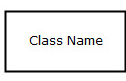
\includegraphics[width=0.17\textwidth]{Figures/table/Sequence/Sequence1}}
		& \setstretch{1.5} {Class แสดงถึงการทำงานของ Use Case ในการส่งหรือรับข้อความ แทนด้วยสัญลักษณ์สี่เหลี่ยมมีชื่อคลาสอยู่ภายใน} \\ \hline
		\raisebox{-\totalheight}{
\includegraphics[height=0.08\textheight]{Figures/table/Sequence/Sequence2}}
		& \setstretch{1.5} {Lifeline หรือเส้นอายุขัย แสดงช่วงเวลาตั้งแต่เริ่มสร้าง object ในคลาสนั้น จนกระทั่ง object นั้นถูกทำลาย สัญลักษณ์แทนด้วยเส้นประ} \\ \hline
		\raisebox{-\totalheight}{
\includegraphics[height=0.08\textheight]{Figures/table/Sequence/Sequence3}}
		& \setstretch{1.5} {Focus of control หรือจุดควบคุม เป็นจุดควบคุมที่ object ใช้ทำการส่งหรือรับข้อความ สัญลักษณ์แทนด้วยสี่เหลี่ยม} \\ \hline
		\raisebox{-\totalheight}{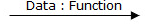
\includegraphics[width=0.3\textwidth]{Figures/table/Sequence/Sequence4}}
		& \setstretch{1.5} {Message คือ ข้อความที่รับส่งระหว่าง Object สัญลักษณ์แทนด้วยลูกศรและประกอบด้วย 2 ส่วน คือ ข้อมูล (Data) และฟังก์ชัน (Function)} \\ \hline
		\raisebox{-\totalheight}{
\includegraphics[width=0.3\textwidth]{Figures/table/Sequence/Sequence5}}
		& \setstretch{1.5} {Return Message เป็นข้อมูลที่ส่งกลับหลังจากทำงานเสร็จ} \\ \hline
		\raisebox{-\totalheight}{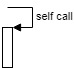
\includegraphics[height=0.08\textheight]{Figures/3/selfcall}}
		& \setstretch{1.5} {Self call เป็นการเรียกฟังชันก์การทำงานภายในตัวเอง} \\ \hline
		\raisebox{-\totalheight}{
\includegraphics[height=0.1\textheight,width=0.3\textwidth]{Figures/3/frame}}
		& \setstretch{1.5} {สร้างกรอบการทำงานของโปรแกรม เพื่อให้รู้ขอบเขตของการทำงานเช่น ลูป(loop)} \\ \hline
		\end{tabular}
	\end{table}
%
%	Sequence Diagram ที่ใช้อธิบายการทำงานของระบบกองทุนเงินให้กู้ยืมเพื่อการศึกษา คณะวิทยสศาสตร์ มหาวิทยาลัยอุบลราชธานี มีรายละเอียดดังต่อไปนี้

\newpage
	\begin{landscape}
	\begin{figure}[H]
		\centering
		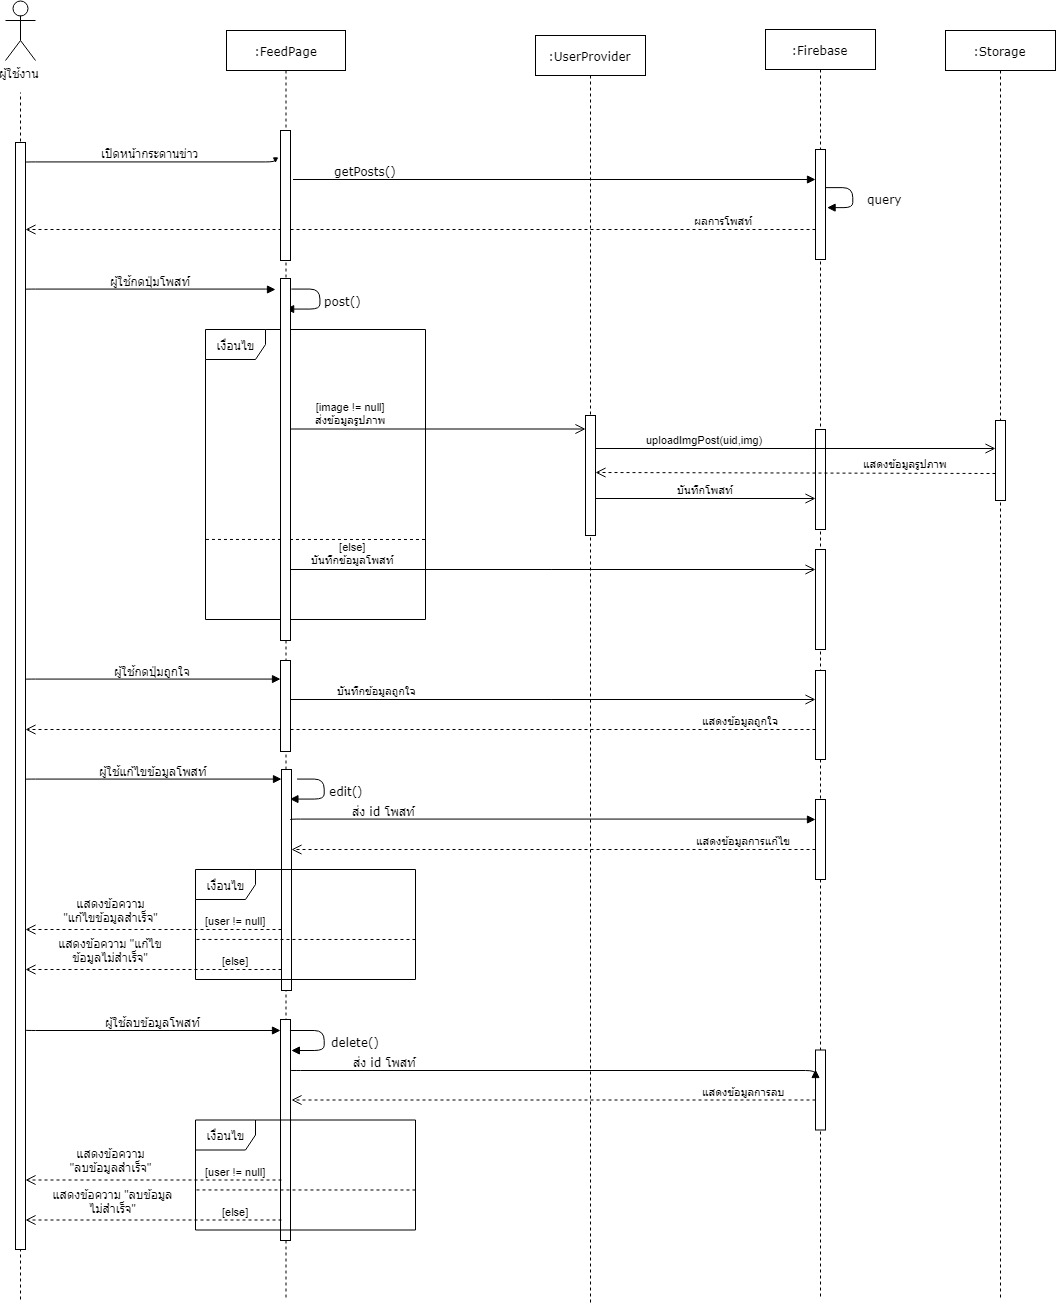
\includegraphics[width=0.95\columnwidth]
		{Figures/3/Sequence/feed}
		\caption{Sequence Diagram การแสดงข่าวสาร}
		\label{Fig:Sequence-feed}
	\end{figure}
  \end{landscape}

	จากภาพที่ \ref{Fig:Sequence-feed} สามารถอธิบายแผนภาพ Sequence Diagram แสดงข่าวสาร ได้ดังนี้ เมื่อ
	ผู้ใช้เปิดโปรแกรมระบบจะเรียกใช้เมธอด onCreate() ที่คลาส MainActivity ระบบจะทำการสร้าง
	Fragment ขึ้นมาโดยใช้เมธอด onCreate() ที่คลาส FeedFragment เมื่อ FeedFragment ถูกติดตั้งบน MainActivity เมธอด callData() จะสืบค้นข้อมูลจากฐานข้อมูลบน Firebase FireStore และส่งข้อมูลที่ได้ไปแปลงที่คลาส FeedItemAdapter โดยมีการคืนค่าเป็นข้อมูลข่าวสารแต่ละแถวและในขั้นตอนสุดท้ายคลาส FeedFragment จะทำการแสดงรายการข้อมูลข่าวสารทั้งหมดออกทางหน้าจอ หากผู้ใช้มีการกดเลือกข่าวสารบางแถวคลาส FeedFragment จะทำการเรียกใช้ PostDetailActivity เพื่อแสดงรายละเอียดข้อมูลข่าวสารของแถวที่ถูกเลือก
	\begin{sidewaysfigure}
	\begin{figure}[H]
		\centering
		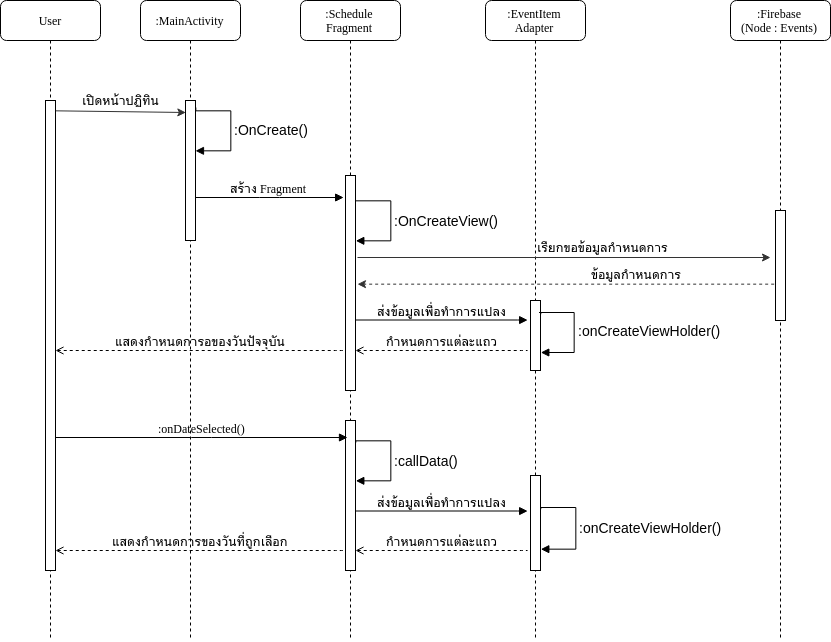
\includegraphics[width=0.8\columnwidth]
		{Figures/3/Sequence/calendar}
		\caption{Sequence Diagram การแสดงปฏิทินกำหนดการ}
		\label{Fig:Sequence-calendar}
	\end{figure}
	\end{sidewaysfigure}
	\newpage
	จากภาพที่ \ref{Fig:Sequence-calendar} สามารถอธิบายแผนภาพ Sequence Diagram แสดงปฏิทินกำหนดการ ได้ดังนี้ เมื่อ
	ผู้ใช้เปิดโปรแกรมระบบจะเรียกใช้เมธอด onCreate() ที่คลาส MainActivity ระบบจะทำการสร้าง
	Fragment ขึ้นมาโดยใช้เมธอด onCreate() ที่คลาส ScheduleFragment เมื่อ ScheduleFragment ถูกติดตั้งบน MainActivity เมธอด callData() จะสืบค้นข้อมูลกำหนดการของวันปัจจุบันจากฐานข้อมูลบน Firebase FireStore และส่งข้อมูลที่ได้ไปแปลงที่คลาส Schedule-ItemAdapter โดยมีการคืนค่าเป็นข้อมูลกำหนดการแต่ละแถวและในขั้นตอนสุดท้ายคลาส Schedule-Fragment จะทำการแสดงรายการกำหนดการวันปัจจุบันออกทางหน้าจอ หากผู้ใช้มีการกดเลือกวันที่ที่ต้องการทราบกำหนดการจากปฏิทินคลาส ScheduleFragment จะทำการเรียกใช้ callData() อีกครั้งโดยสืบค้นข้อมูลกำหนดการของวันที่ถูกเลือกจากฐานข้อมูลบน Firebase FireStore และส่งข้อมูลที่ได้ไปแปลงที่คลาส ScheduleItemAdapter โดยมีการคืนค่าเป็นข้อมูลแต่กำหนดการละแถวและในขั้นตอนสุดท้ายคลาส ScheduleFragment จะทำการแสดงรายการกำหนดการวันที่ผู้ใช้เลือกออกทางหน้าจอ

	\begin{sidewaysfigure}
	\begin{figure}[H]
		\centering
		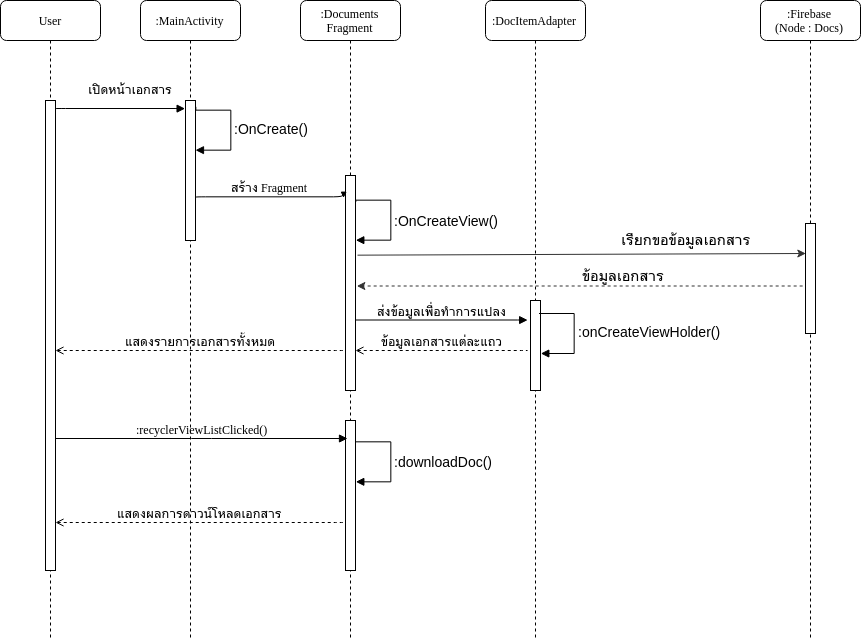
\includegraphics[width=0.8\columnwidth]
		{Figures/3/Sequence/doc}
		\caption{Sequence Diagram การแสดงดาวน์โหลดเอกสาร}
		\label{Fig:Sequence-doc}
	\end{figure}
	\end{sidewaysfigure}
	\newpage
	จากภาพที่ \ref{Fig:Sequence-doc} สามารถอธิบายแผนภาพ Sequence Diagram แสดงดาวน์โหลดเอกสาร ได้ดังนี้ เมื่อผู้ใช้เปิดโปรแกรมระบบจะเรียกใช้เมธอด onCreate() ที่คลาส MainActivity ระบบจะทำการสร้าง
	Fragment ขึ้นมาโดยใช้เมธอด onCreate() ที่คลาส DocumentsFragment เมื่อ DocumentsFragment ถูกติดตั้งบน MainActivity เมธอด initInstances() จะสืบค้นข้อมูลเอกสารทั้งหมดจากฐานข้อมูลบน Firebase FireStore และส่งข้อมูลที่ได้ไปแปลงที่คลาส DocItem-Adapter โดยมีการคืนค่าเป็นข้อมูลเอกสารแต่ละแถวและในขั้นตอนสุดท้ายคลาส Documents-Fragment จะทำการแสดงรายการกำหนดการวันปัจจุบันออกทางหน้าจอ

	\begin{sidewaysfigure}
	\begin{figure}[H]
		\centering
		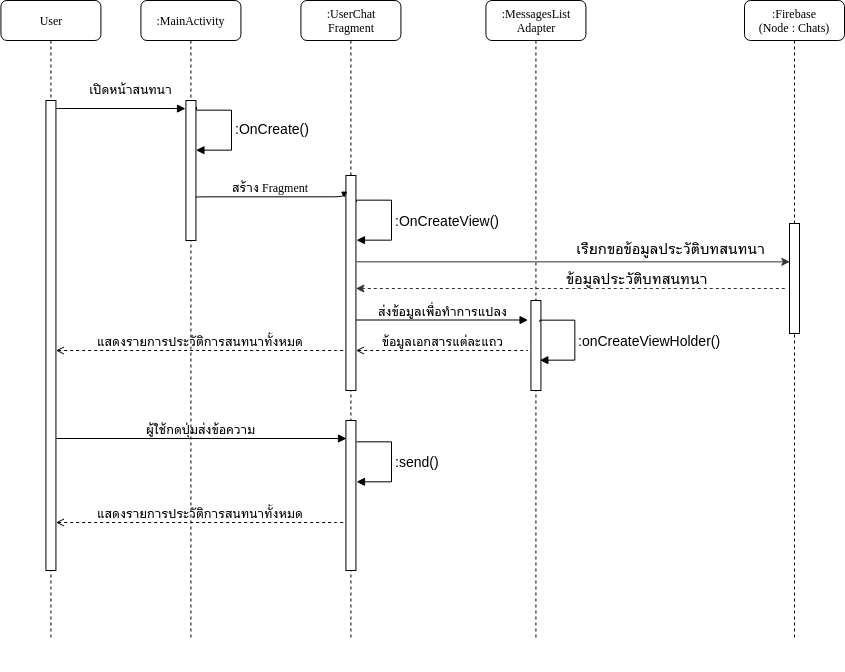
\includegraphics[width=0.8\columnwidth]
		{Figures/3/Sequence/chat}
		\caption{Sequence Diagram การแสดงบทสนทนา}
		\label{Fig:Sequence-chat}
	\end{figure}
	\end{sidewaysfigure}
	\newpage
	จากภาพที่ \ref{Fig:Sequence-chat} สามารถอธิบายแผนภาพ Sequence Diagram แสดงการสนทานา ได้ดังนี้ เมื่อผู้ใช้เปิดโปรแกรมระบบจะเรียกใช้เมธอด onCreate() ที่คลาส MainActivity ระบบจะทำการสร้าง
	Fragment ขึ้นมาโดยใช้เมธอด onCreate() ที่คลาส UserChatFragment เมื่อ UserChatFrag-ment ถูกติดตั้งบน MainActivity เมธอด getMessage() จะสืบค้นข้อมูลประวัติการสนทนาของผู้ใช้คนปัจจุบันทั้งหมดจากฐานข้อมูลบน Firebase FireStore และส่งข้อมูลที่ได้ไปแปลงที่คลาส MessagesListAdapter โดยมีการคืนค่าเป็นข้อมูลรายการประวัติการสนทนาทั้งหมดและในขั้นตอนสุดท้ายคลาส User-ChatFragment จะทำการแสดงรายการประวัติการสนทนาทั้งหมดออกทางหน้าจอ เมื่อผู้ใช้พิมพ์ข้อความและกดปุ่มส่งระบบจะเรียกให้เมธอด send() เพื่อทำการบันทึกข้อมูลไว้บน Firebase FireStore และทำการแสดงข้อมูลรายการประวัติการสนทนาทั้งหมดที่ถูกอัพเดท

	\begin{sidewaysfigure}
	\begin{figure}[H]
		\centering
		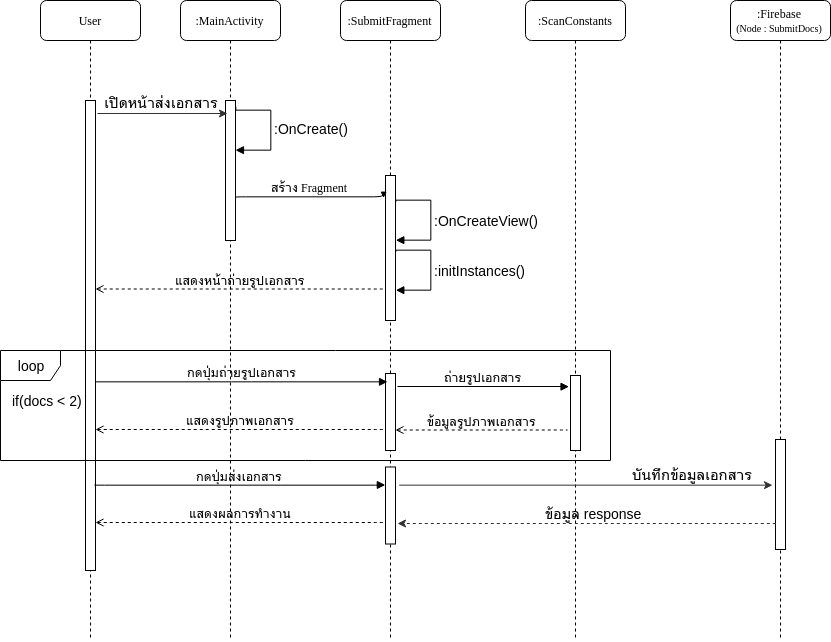
\includegraphics[width=0.8\columnwidth]
		{Figures/3/Sequence/submit}
		\caption{Sequence Diagram แสดงส่งเอกสารตรวจสอบ}
		\label{Fig:Sequence-submit}
	\end{figure}
	\end{sidewaysfigure}
	\newpage
	จากภาพที่ \ref{Fig:Sequence-submit} สามารถอธิบายแผนภาพ Sequence Diagram แสดงส่งเอกสารตรวจสอบ ได้ดังนี้ เมื่อผู้ใช้เปิดโปรแกรมระบบจะเรียกใช้เมธอด onCreate() ที่คลาส MainActivity ระบบจะทำการสร้าง
	Fragment ขึ้นมาโดยใช้เมธอด onCreate() ที่คลาส SubmitFragment เมื่อ Submit-Fragment ถูกติดตั้งบน MainActivity เมธอด initInstances() จะถูกเรียกเพื่อสร้างหน้าจอแสงดผลเมื่อผู้ใช้กดปุ่มถ่ายรูประบบจะเรียกใช้ไลบรารี่ ScanConstants เพื่อถ่ายภาพเอกสารและรอให้ผู้ใช้ถ่ายครบทั้งสองแผ่นจึงจะแสดงปุ่มกดส่งเอกสารเพื่อตรวจสอบ
\newpage	 
	
\section{โครงสร้างฐานข้อมูลไฟร์เบส(Firebase Database Stucture)}
Firebase Database นั้นเป็น Database แบบ NoSQL และเป็น JSON database ที่มีโครงสร้างที่เป็น Key และ Value จัดเก็บข้อมูลในลักษณะโหนด หากต้องการเรียกงานจะเรียกใช้โดย
การท่องไปยังโหนดที่ต้องการ ส่วนประกอบสัญลักษณ์ที่ใช้ในการเขียนโครงสร้างฐานข้อมูลแบบ Firebase
แสดงดังตารางที่ \ref{tab:DB}

\begin{table}[H]
	\centering
	\caption{สัญลักษณ์ของโครงสร้างฐานข้อมูลแบบ Firebase}
	\label{tab:DB}
	\begin{tabular}{| c	| p{10cm} |}
		\hline
		\textbf{สัญลักษณ์} & \multicolumn{1}{c|}{\textbf{คำอธิบาย}} \\ \hline
		\raisebox{-\totalheight}{
\includegraphics[width=0.1\textwidth]{Figures/3/DB/dbroot}}
		& \setstretch{1.5} {Database เป็นการเรียกชื่อแทนโหนด(Node)บนสุดที่ใช้ในการเก็บข้อมูล} \\ \hline
		\raisebox{-\totalheight}{
\includegraphics[width=0.1\textwidth]{Figures/3/DB/dbcollection}}
		& \setstretch{1.5} {Collection เป็นการเรียกชื่อแทนของการเก็บหลาย ๆ เอกสารไว้ด้วยกัน} \\ \hline
		\raisebox{-\totalheight}{
\includegraphics[width=0.1\textwidth]{Figures/3/DB/dbdoc}}
		& \setstretch{1.5} {Document เป็นการเรียกชื่อแทนหน่วยการเก็บของข้อมูลใน Cloud Firestore ภายในจะประกอบไปด้วย ชื่อของ Document  ชื่อของคีย์ (key) และ ค่าข้อมูล (value) โดยชื่อของ Document ห้ามซ้ำกัน ซึ่งใน Cloud Firestore สามารถระบุประเภทของข้อมูลได้ 9 ประเภทได้แก่ boolean, number, string, geo point, timestamp, array, object, reference และ null} \\ \hline
	\end{tabular}
\end{table}
	\begin{figure}[H]
	\centering
	
\includegraphics[width=0.7\columnwidth]
	{Figures/3/DB/DB1}
	\caption{โครงสร้างฐานข้อมูลแบบ Firebase}
	\label{Fig:DB1}
	\end{figure}

	\begin{figure}[H]
	\centering
	
\includegraphics[width=0.9\columnwidth]
	{Figures/3/DB/DB2}
	\caption{โครงสร้างฐานข้อมูลแบบ Firebase(ต่อ)}
	\label{Fig:DB2}
\end{figure}
	\begin{figure}[H]
	\centering
	\includegraphics[width=0.55\columnwidth]
	{Figures/3/DB/DB3}
	\caption{โครงสร้างฐานข้อมูลแบบ Firebase(ต่อ)}
	\label{Fig:DB3}
\end{figure}
	\begin{figure}[H]
	\centering
	\includegraphics[width=0.7\columnwidth]
	{Figures/3/DB/DB4}
	\caption{โครงสร้างฐานข้อมูลแบบ Firebase(ต่อ)}
	\label{Fig:DB4}
\end{figure}

\newpage
จากรูที่ \ref{Fig:DB1}-\ref{Fig:DB4} สามารถอธิบายโครงสร้างของข้อมูลได้ดังนี้
\begin{figure}[H]
\centering
\includegraphics[width=0.5\columnwidth]
{Figures/3/DB/nodePost}
\caption{โหนดเก็บข้อมูลประกาศ}
\label{Fig:DB4}
\end{figure}
\begin{table}[H]
	\centering
	\caption{อธิบายโหนดที่ใช้เก็บข้อมูลประกาศ}
	\label{my-label1}
	\begin{tabular}{|c|p{10cm}|}
		\hline
		\multicolumn{1}{|c|}{\textbf{Key}} & \multicolumn{1}{c|}{\textbf{คำอธิบาย}} \\ \hline
		Posts & โหนดสำหรับเก็บข้อมูลประกาศทั้งหมด \\ \hline
		Post &  สำหรับเก็บข้อมูลแต่ละประกาศ \\ \hline
		title & สำหรับเก็บชื่อหัวข้อประกาศ \\ \hline
		description & สำหรับเก็บรายละเอียดประกาศ  \\ \hline
		collection & สำหรับเก็บประเภทของประกาศได้แก่ สาธารณะและเฉพาะบุคคล \\ \hline
		fileURL & สำหรับเก็บ url ของเอกสารแนบประกาศ \\ \hline
		id & สำหรับเก็บรหัสของประกาศ \\ \hline
		time & สำหรับเก็บเวลาที่ประกาศ \\ \hline
	\end{tabular}
\end{table}

\newpage
\begin{figure}[H]
	\centering
	\includegraphics[width=0.5\columnwidth]
	{Figures/3/DB/nodeDoc}
	\caption{โหนดเก็บข้อมูลเอกสารที่เกี่ยวข้อง}
	\label{Fig:DB4}
\end{figure}
\begin{table}[H]
	\centering
	\caption{อธิบายโหนดที่ใช้เก็บข้อมูลเอกสารที่เกี่ยวข้อง}
	\label{my-label1}
	\begin{tabular}{|c|p{10cm}|}
		\hline
		\multicolumn{1}{|c|}{\textbf{Key}} & \multicolumn{1}{c|}{\textbf{คำอธิบาย}} \\ \hline
		Docs & โหนดสำหรับเก็บข้อมูลของเอกสารที่เกี่ยวข้องทั้งหมด \\ \hline
		Doc &  สำหรับเก็บข้อมูลเอกสารแต่ละฉบับ \\ \hline
		title & สำหรับเก็บชื่อหัวเรื่องของเอกสาร \\ \hline
		description & สำหรับเก็บรายละเอียดของเอกสาร \\ \hline
		fileType & สำหรับนามสกุลไฟล์เอกสาร เช่น .pdf .png เป็นต้น \\ \hline
		fileURL & สำหรับเก็บ url ของเอกสาร\\ \hline
		time & สำหรับเก็บเวลาที่ถูกอัพโหลดเข้าสู่ระบบโดยเจ้าหน้าที่\\ \hline
	\end{tabular}
\end{table}

\newpage
\begin{figure}[H]
	\centering
	\includegraphics[width=0.4\columnwidth]
	{Figures/3/DB/nodeChat}
	\caption{โหนดเก็บข้อมูลประวัติการสนทนา}
	\label{Fig:DB4}
\end{figure}
\begin{table}[H]
	\centering
	\caption{อธิบายโหนดที่ใช้เก็บข้อมูลประวัติการสนทนา}
	\label{my-label1}
	\begin{tabular}{|c|p{10cm}|}
		\hline
		\multicolumn{1}{|c|}{\textbf{Key}} & \multicolumn{1}{c|}{\textbf{คำอธิบาย}} \\ \hline
		Chats & โหนดสำหรับเก็บข้อมูลประวัติการสนทนาทั้งหมด \\ \hline
		User\_id &  สำหรับเก็บประวัติการสนทนาของผู้ใช้แต่ละคน \\ \hline
		Messages & สำหรับเก็บประวัติการสนทนาทั้งหมดของผู้ใช้ \\ \hline
		Message & สำหรับเก็บข้อมูลของแต่ละข้อความ \\ \hline
		message & สำหรับเก็บข้อความ \\ \hline
		name & สำหรับเก็บชื่อของผู้ส่งข้อความ\\ \hline
		photo & สำหรับเก็บ url รูปภาพของผู้ส่งข้อความ\\ \hline
		senderId & สำหรับเก็บรหัสของผู้ส่งข้อความ\\ \hline
		time & สำหรับเก็บเวลาที่ข้อความถูกส่ง\\ \hline
	\end{tabular}
\end{table}

\newpage
\begin{figure}[H]
	\centering
	\includegraphics[width=0.5\columnwidth]
	{Figures/3/DB/nodeEvent}
	\caption{โหนดเก็บข้อมูลกำหนดการ}
	\label{Fig:DB4}
\end{figure}
\begin{table}[H]
	\centering
	\caption{อธิบายโหนดที่ใช้เก็บข้อมูลกำหนดการ}
	\label{my-label1}
	\begin{tabular}{|c|p{10cm}|}
		\hline
		\multicolumn{1}{|c|}{\textbf{Key}} & \multicolumn{1}{c|}{\textbf{คำอธิบาย}} \\ \hline
		Events & โหนดสำหรับเก็บข้อมูลของกำหนดการทั้งหมด \\ \hline
		Event & สำหรับเก็บข้อมูลของแต่ละกำหนดการ \\ \hline
		title & สำหรับเก็บชื่อหัวข้อของกำหนดการ \\ \hline
		description & สำหรับเก็บรายละเอียดของกำหนดการ\\ \hline
		time & สำหรับเก็บเวลาของกำหนดการ\\ \hline
	\end{tabular}
\end{table}

\newpage
\begin{figure}[H]
	\centering
	\includegraphics[width=0.4\columnwidth]
	{Figures/3/DB/nodeReq}
	\caption{โหนดเก็บข้อมูลการยื่นสำเนาเอกสารเพื่อตรวจสอบของนักศึกษา}
	\label{Fig:DB4}
\end{figure}
\begin{table}[H]
	\centering
	\caption{อธิบายโหนดที่ใช้เก็บข้อมูลการยื่นสำเนาเอกสารเพื่อตรวจสอบของนักศึกษา}
	\label{my-label1}
	\begin{tabular}{|c|p{10cm}|}
		\hline
		\multicolumn{1}{|c|}{\textbf{Key}} & \multicolumn{1}{c|}{\textbf{คำอธิบาย}} \\ \hline
		RusetSubmitDocs & โหนดสำหรับเก็บข้อมูลการยื่นสำเนาเอกสารเพื่อตรวจสอบของนักศึกษาทั้งหมด \\ \hline
		User\_id & สำหรับเก็บข้อมูลของแต่ละสำเนาเอกสารของนักศึกษาแต่ละคน \\ \hline
		doc2 & สำหรับเก็บ url ของภาพถ่ายสำเนาเอกสารฉบับที่ 1\\ \hline
		doc2 & สำหรับเก็บ url ของภาพถ่ายสำเนาเอกสารฉบับที่ 2\\ \hline
		status & สำหรับเก็บผลการตรวจสอบของเจ้าหน้าที่ \\ \hline
		time & สำหรับเก็บเวลาที่สำเนาเอกสารถูกเพิ่มเข้าสู่ระบบ \\ \hline
	\end{tabular}
\end{table}

\newpage
\begin{figure}[H]
	\centering
	\includegraphics[width=0.35\columnwidth]
	{Figures/3/DB/nodeUser}
	\caption{โหนดเก็บข้อมูลของนักศึกษา}
	\label{Fig:DB4}
\end{figure}
\begin{table}[H]
	\centering
	\caption{อธิบายโหนดที่ใช้เก็บข้อมูลของนักศึกษา}
	\label{my-label1}
	\begin{tabular}{|c|p{10cm}|}
		\hline
		\multicolumn{1}{|c|}{\textbf{Key}} & \multicolumn{1}{c|}{\textbf{คำอธิบาย}} \\ \hline
		Users & โหนดสำหรับเก็บข้อมูลของนักศึกษา \\ \hline
		User\_id & สำหรับเก็บข้อมูลของนักศึกษาแต่ละคน \\ \hline
		depart & สำหรับเก็บภาควิชาของนักศึกษา\\ \hline
		major & สำหรับเก็บสาขาของนักศึกษา\\ \hline
		sid & สำหรับเก็บรหัสประจำตัวนักศึกษา \\ \hline
		name & สำหรับเก็บชื่อของนักศึกษา \\ \hline
		year & สำหรับเก็บชั้นปีของนักศึกษา \\ \hline
		lastChat & สำหรับเก็บเวลาที่สนทนากับเจ้าหน้าที่ล่าสุด \\ \hline
		photoUrl & สำหรับเก็บ url รูปภาพโปรไฟล์ (Profile) \\ \hline
	\end{tabular}
\end{table}

\newpage
\begin{figure}[H]
	\centering
	\includegraphics[width=0.5\columnwidth]
	{Figures/3/DB/nodeQueue}
	\caption{โหนดเก็บข้อมูลการจองคิวของนักศึกษา}
	\label{Fig:DB4}
\end{figure}
\begin{table}[H]
	\centering
	\caption{อธิบายโหนดที่ใช้เก็บข้อมูลการจองคิวของนักศึกษา}
	\label{my-label1}
	\begin{tabular}{|c|p{10cm}|}
		\hline
		\multicolumn{1}{|c|}{\textbf{Key}} & \multicolumn{1}{c|}{\textbf{คำอธิบาย}} \\ \hline
		Queue & โหนดสำหรับเก็บข้อมูลการจองคิวของนักศึกษาทั้งหมด \\ \hline
		q\_id &  สำหรับเก็บข้อมูลของการจองคิวแต่ละครั้งที่เปิดจองคิว \\ \hline
		Date &  สำหรับเก็บวันที่สำหรับส่งเอกสาร\\ \hline
		Time &  สำหรับเก็บรายชื่อของนักศึกษาที่ทำการจองคิวในส่งเอกสารเวลานั้น ๆ\\ \hline
		User\_id & สำหรับเก็บรหัสของนักศึกษา \\ \hline
		title & สำหรับเก็บชื่อหัวเรื่องกำหนดการการจองคิว \\ \hline
		studentPerHr & สำหรับเก็บจำนวนนักศึกษาต่อชั่วโมง \\ \hline
	\end{tabular}
\end{table}

\newpagedr
\begin{figure}[H]
	\centering
	\includegraphics[width=0.4\columnwidth]
	{Figures/3/DB/nodeFaq}
	\caption{โหนดเก็บข้อมูลคำถามที่พบบ่อย}
	\label{Fig:DB4}
\end{figure}
\begin{table}[H]
	\centering
	\caption{อธิบายโหนดที่ใช้เก็บข้อมูลคำถามที่พบบ่อย}
	\label{my-label1}
	\begin{tabular}{|c|p{10cm}|}
		\hline
		\multicolumn{1}{|c|}{\textbf{Key}} & \multicolumn{1}{c|}{\textbf{คำอธิบาย}} \\ \hline
		Queue & โหนดสำหรับเก็บข้อมูลคำถามที่พบบ่อยทั้งหมด \\ \hline
		Faq\_id & สำหรับเก็บข้อมูลคำถามที่พบบ่อยแต่ละรายการ \\ \hline
		title & สำหรับเก็บคำถาม \\ \hline
		description & สำหรับเก็บคำตอบ \\ \hline
	\end{tabular}
\end{table}
